\section{Experiments}\label{sec:experiments}
In this section, we empirically evaluate the performance of different components we discussed throughout the paper. More specifically, (1) we first focus on the presented optimization algorithms and compare them with state-of-the-art methods; (2) We then focus on in-context and continual learning tasks and show how the nested learning paradigm and more specifically higher order in-context learning enhances the capabilities of models. We compare the continuum memory system with simple MLP layers and discuss how a pre-trained model can be adapted to be a continual learner; (3) We then focus on the language modeling and long context understanding of \model{} model and compare it with Transformers and modern recurrent architectures. The details of the experiments and their setups are explained in the corresponding sections.  




\begin{figure*}
    \centering
    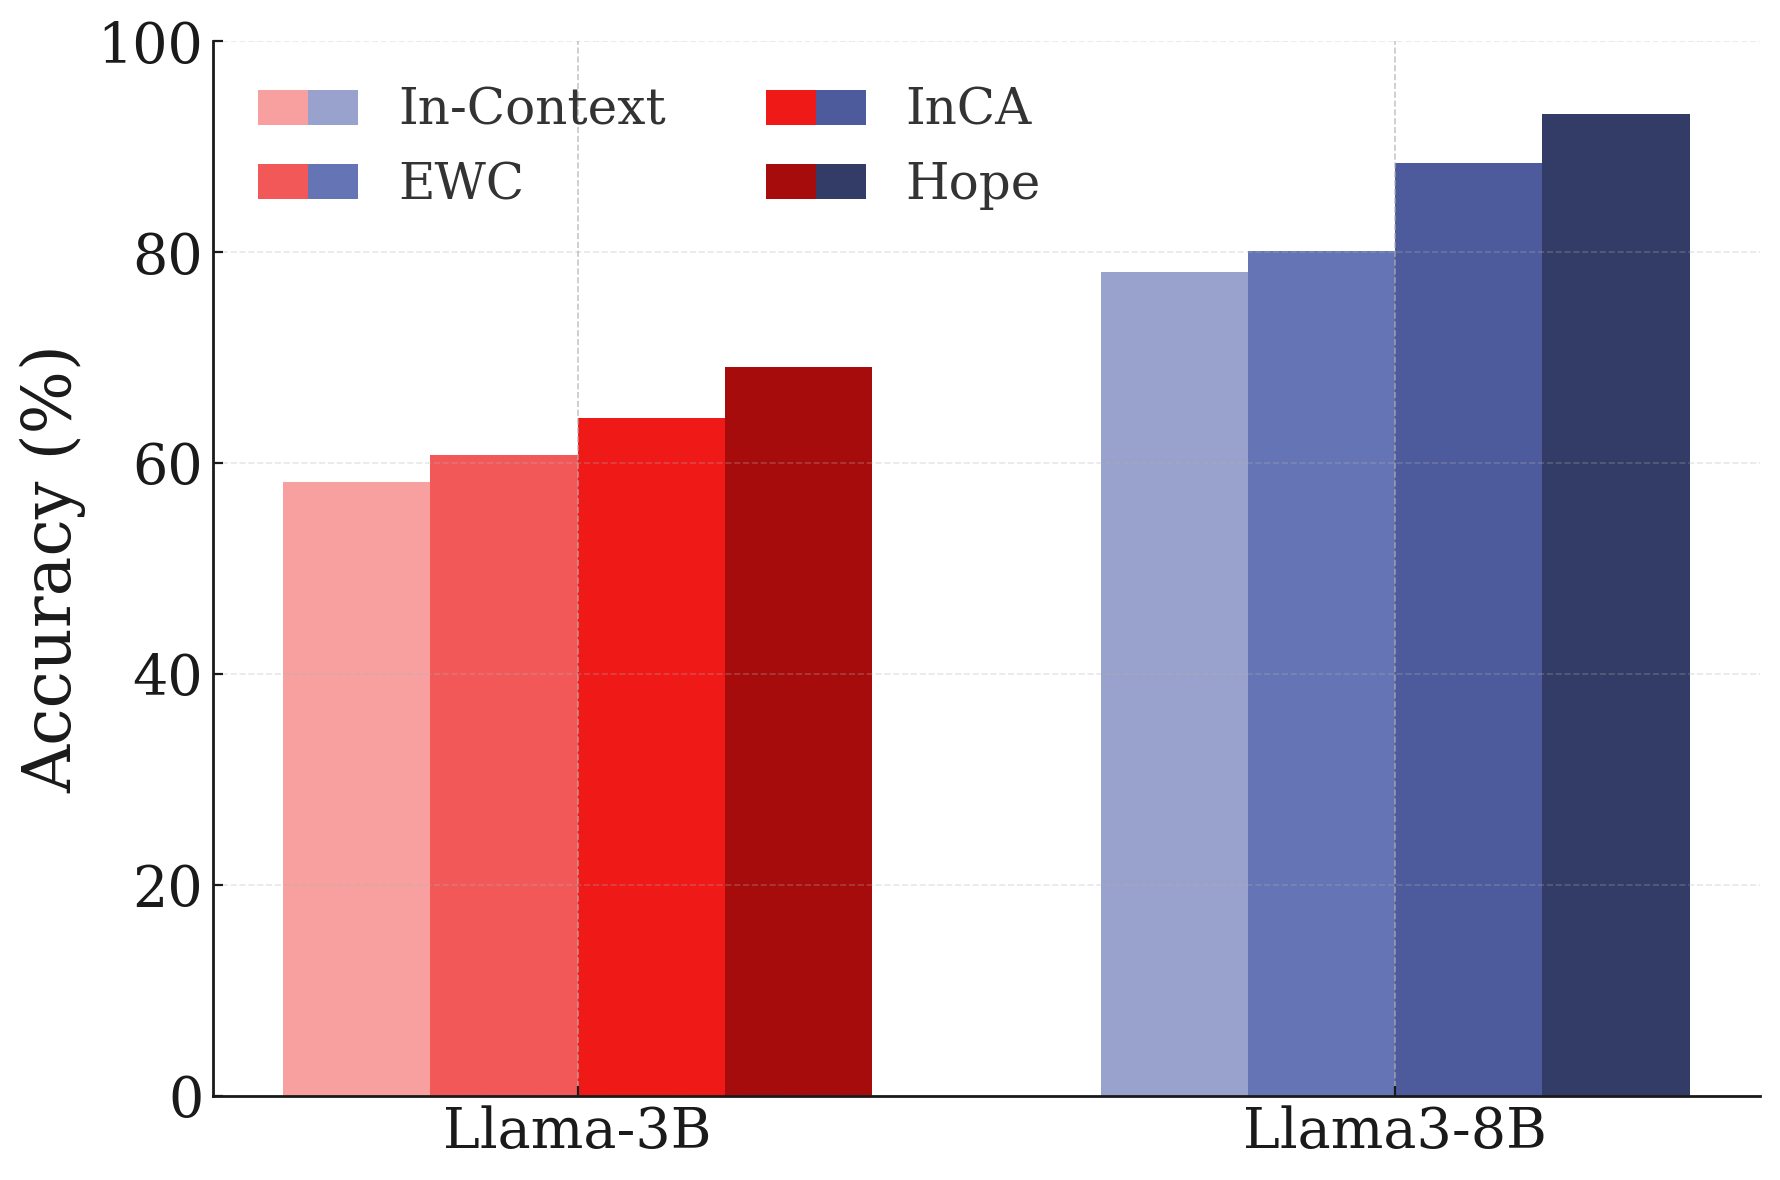
\includegraphics[width=0.31\linewidth]{Images/CLINC.png}~\hfill~
    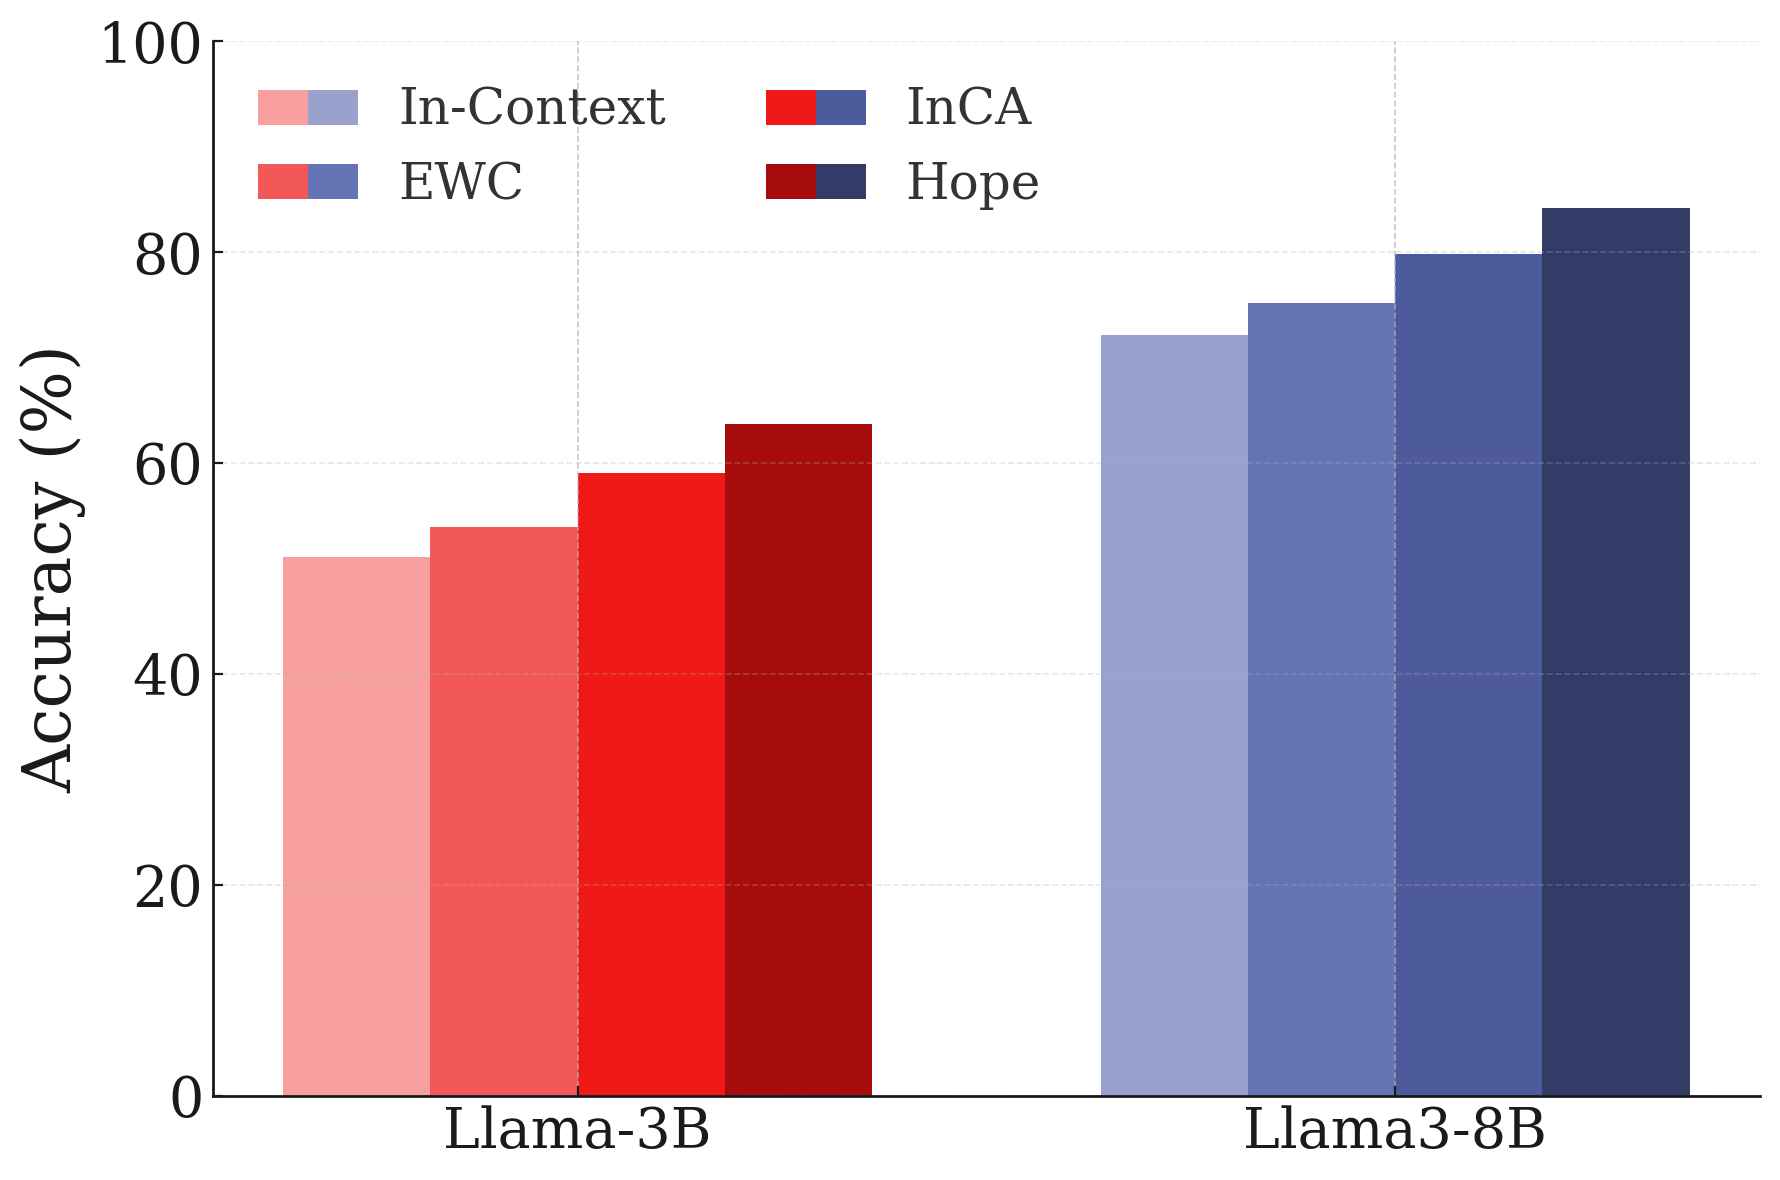
\includegraphics[width=0.31\linewidth]{Images/Banking.png}~\hfill~
    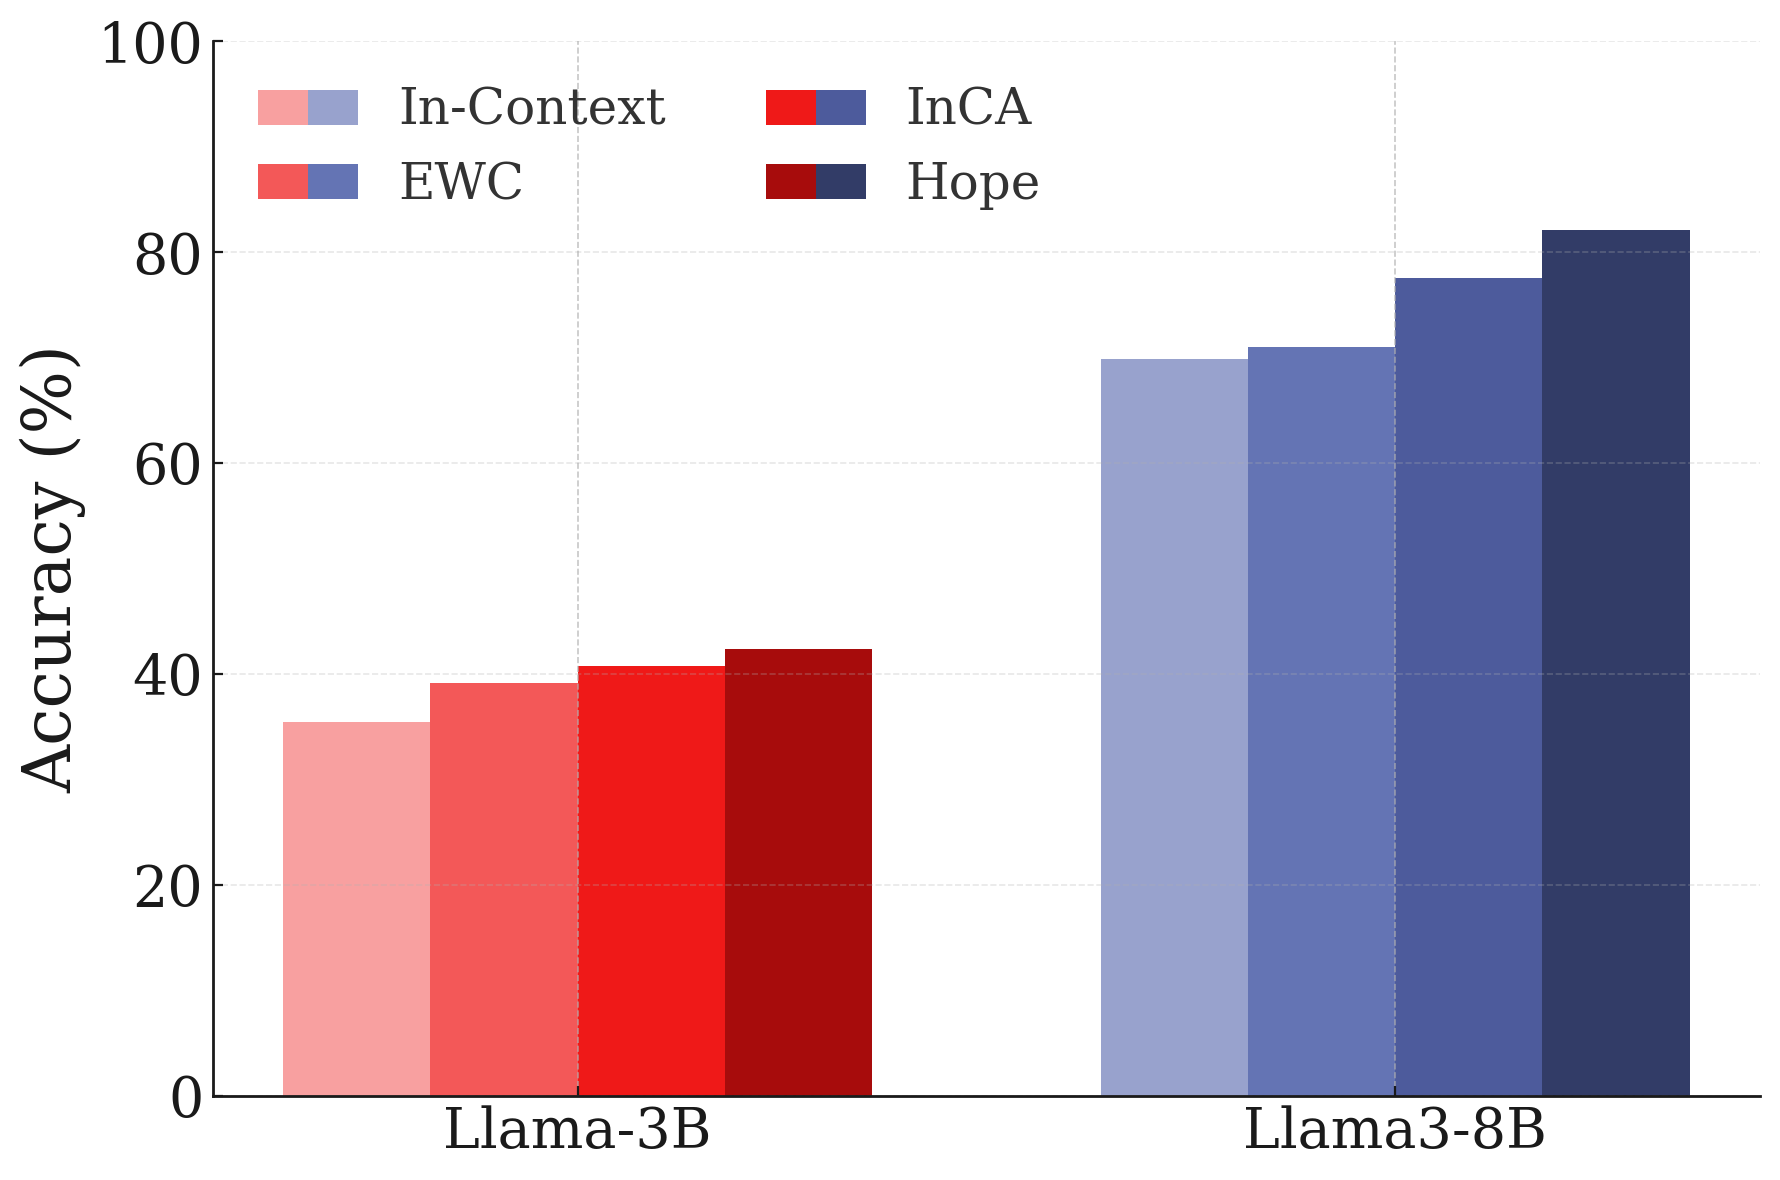
\includegraphics[width=0.31\linewidth]{Images/DBpedia.png}
    \caption{Class-incremental learning in the text classification domain on (Left) CLINC dataset~\citep{larson2019evaluation}, (Middle) Banking dataset~\citep{casanueva2020efficient}, and (Right) DBpedia dataset~\citep{auer2007dbpedia}. \model-enhanced architecture achieves the best accuracy among other continual learning methods, including ICL.}
    \label{fig:CIL}
\end{figure*}


\begin{figure*}
    \centering
    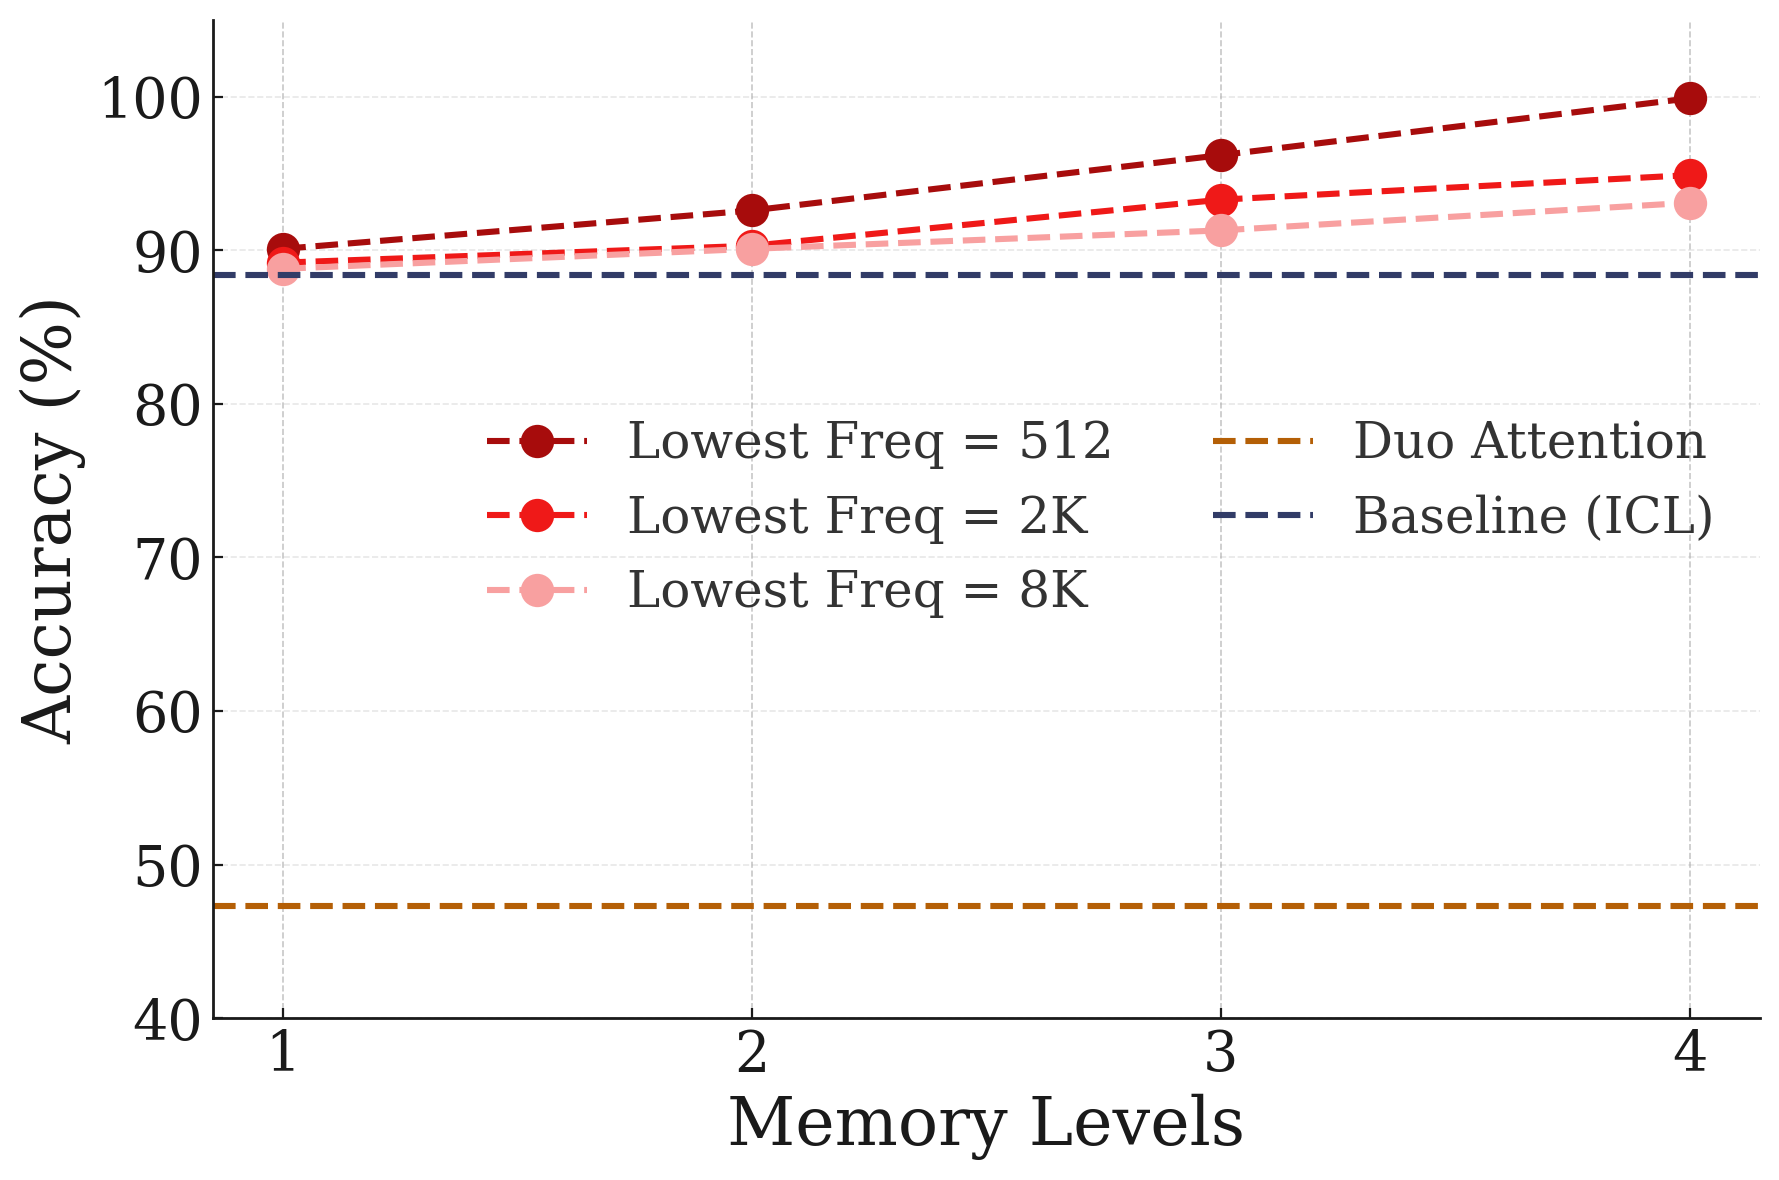
\includegraphics[width=0.33\linewidth]{Images/NIAH-levels.png}
    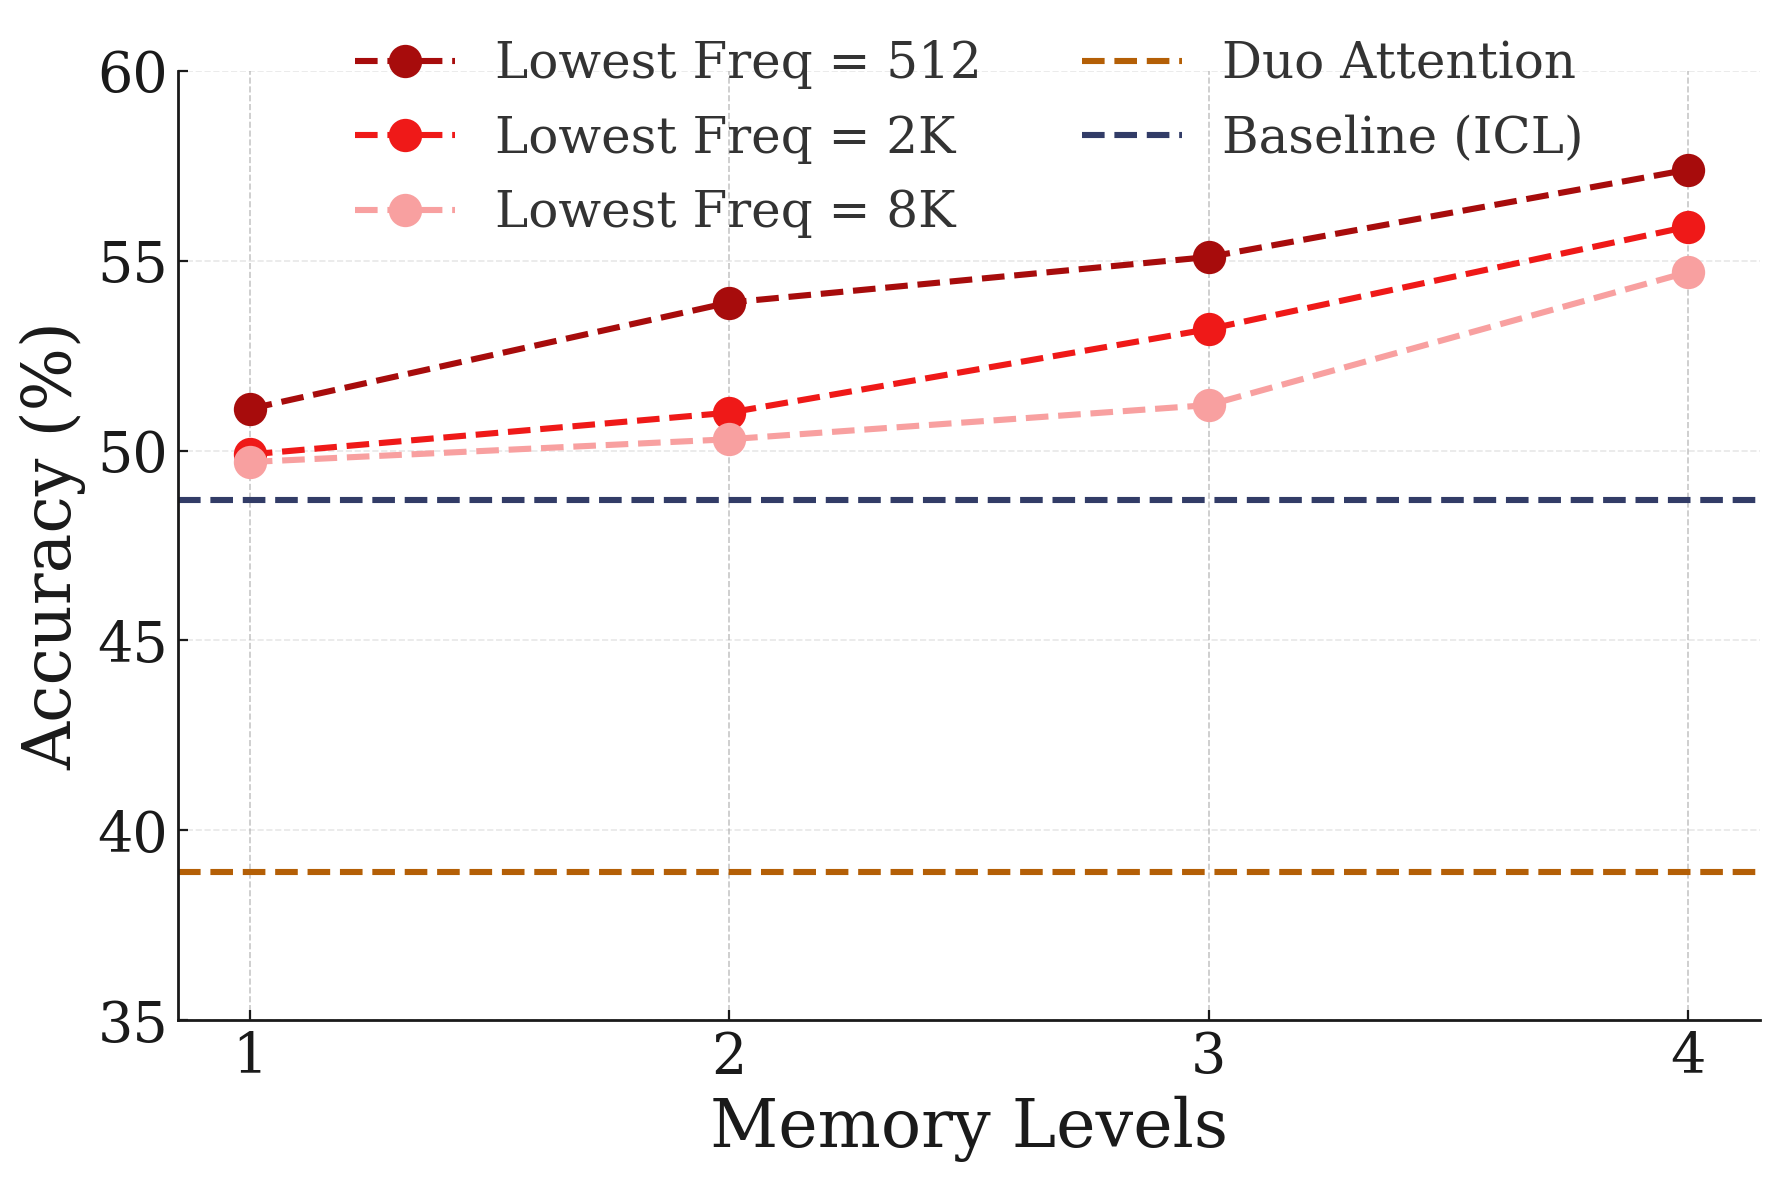
\includegraphics[width=0.33\linewidth]{Images/LongHelath-levels.png}
    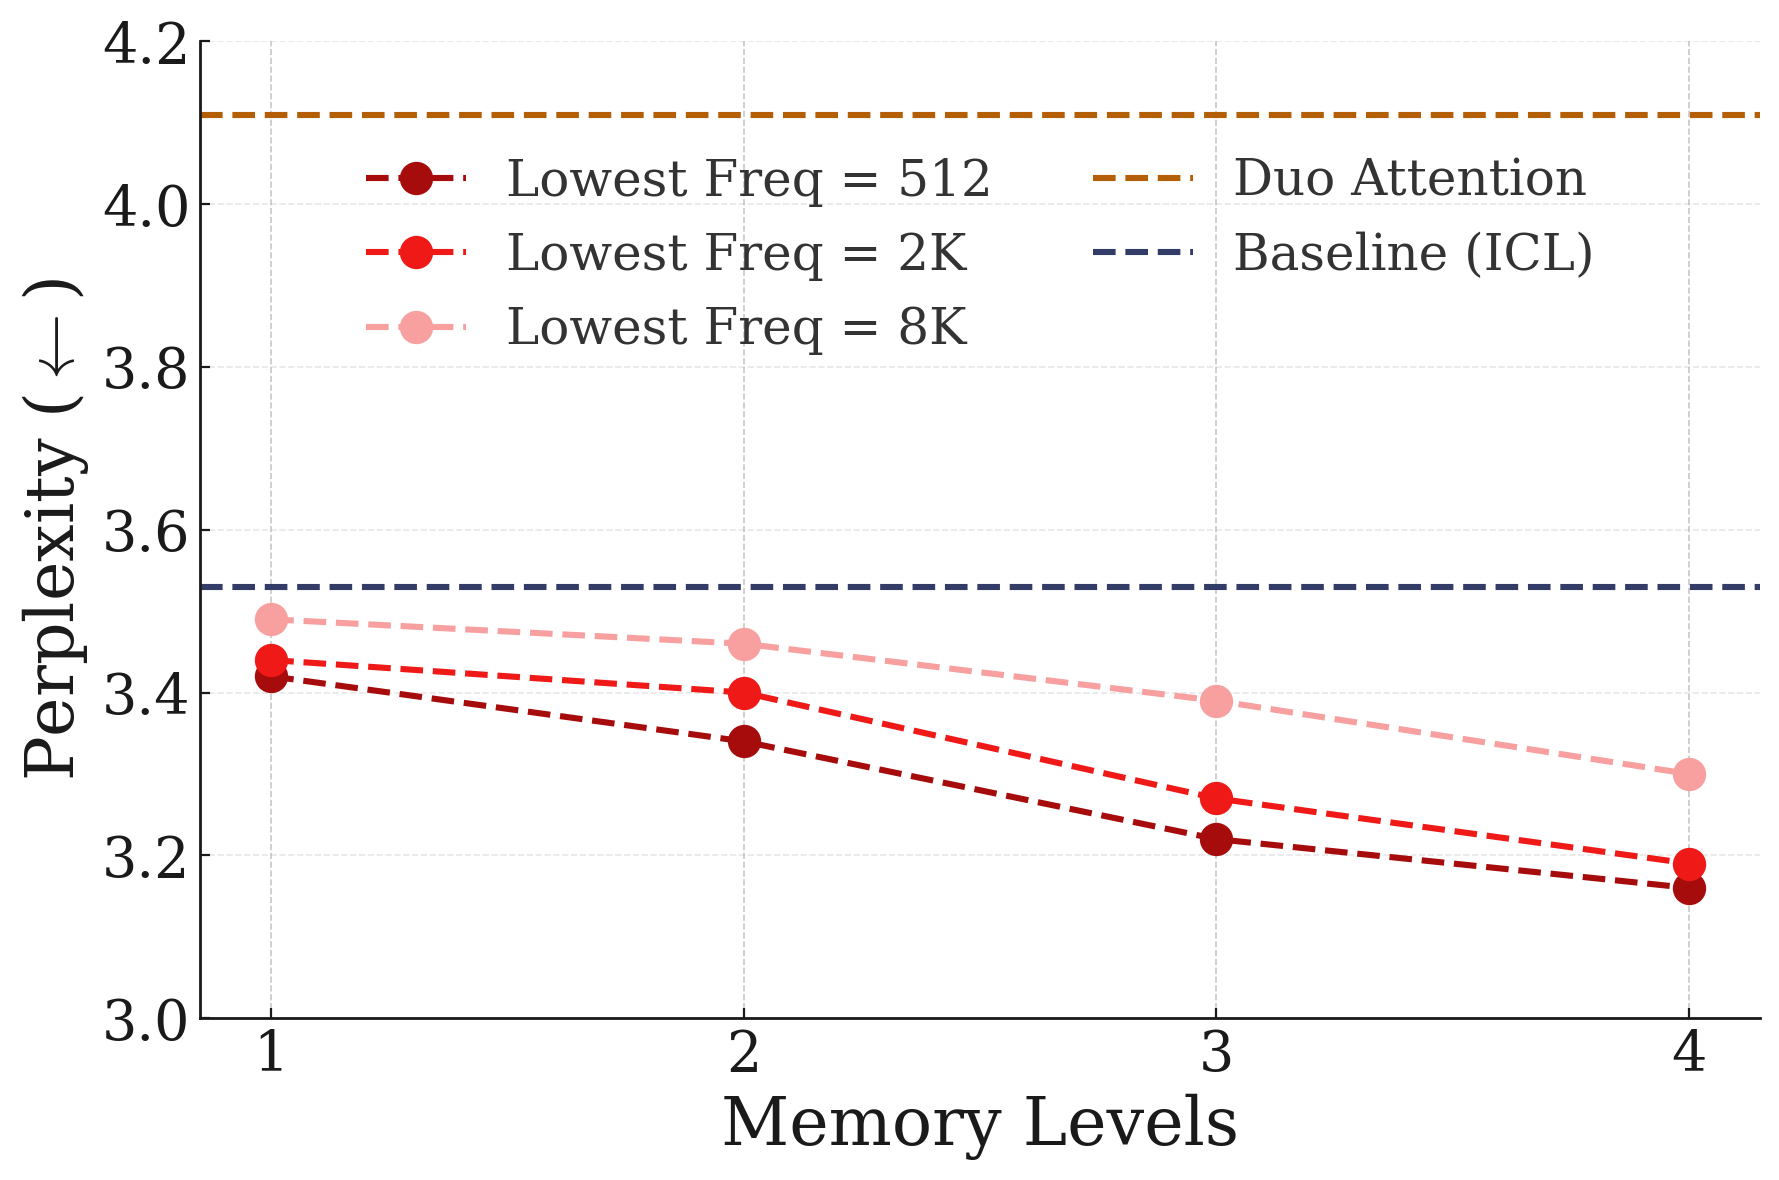
\includegraphics[width=0.33\linewidth]{Images/QASPER-levels.png}
    \caption{The effect of memory levels on the in-context learning performance of the model in (Left) MK-NIAH of RULER~\citep{hsieh2024ruler}, (Middle) LongHealth~\citep{adams2025longhealth}, (Right) QASPER~\citep{dasigi2021dataset} benchmarks. Note that for QASPER benchmark (Right), the lower values indicate better performance.}
    \label{fig:effect-level}
\end{figure*}




\subsection{\model: Continual Learning and Long Context Understanding}
One of the main goals of NL is to enhance the continual learning capabilities, and so in this section, we evaluate NL and its implications such as Continuum Memory System (CMS) and \model{} on multiple continual learning and long context understanding tasks. For each of the tasks, we use the best reported results on the benchmark as the baselines.






\head{Class Incremental Learning}
First, we focus on class-incremental learning tasks on three datasets: 
\begin{itemize}
    \item CLINC~\citep{larson2019evaluation}: CLINC is a multi-domain intent classification benchmark designed for task-oriented dialog systems, with a special focus on detecting out-of-scope (OOS) queries. It has 150 in-scope intent classes spanning 10 broad domains (e.g. Banking, Travel, Home, Weather, Small Talk, etc.) with 23.7K total queries, of which 22.5K are in-scope and 1.2K are out-of-scope. 
    \item Banking~\citep{casanueva2020efficient}: Banking dataset is a single-domain intent classification benchmark focused on fine-grained customer service queries in the banking domain. In this dataset, each example is a short customer query (e.g. “How can I reset my card PIN?”) that must be classified into the correct banking intent/category. There are 3083 total examples labeled with the 77 intents (heavily imbalanced classes).
    \item DBpedia~\citep{auer2007dbpedia}: DBpedia is a text classification benchmark from Wikipedia where article abstracts are expected to be categorized into ontology topic classes. In other words, given a short Wikipedia description, the goal is to predict its high-level topic/category (such as whether the article is about a book, a film, an animal, a place, etc.). The dataset has over 340K examples labeled across those 70 second-level classes, but we sample 10K training and 1K test instances for the 70-class DBpedia task.
\end{itemize}
As the backbone of our \model{} models we use Llama3-8B and Llama-3B~\citep{dubey2024llama}, and then employ our technique discussed in \autoref{sec:pre-trained-mlp} to make the MLP blocks capable of adaption, placing them in different levels with different frequency updates followed by continual pre-training with 15B tokens. Following \citet{momeni2025context}, we use simple in-context learning (ICL) capability of Llama-3 models (with the same process of continual pre-training with 15B tokens but without any change in the MLP blocks), Elastic Weight Consolidation (EWC)~\citep{kirkpatrick2017overcoming}, and In-context
Continual Learning with an External Learner (InCA)~\citep{momeni2025context}  as the baselines of our evaluation. The results are reported in \autoref{fig:CIL}. \model{} shows the best performance across all continual learning baselines, including models with external learner (i.e., InCA). Comparing \model{} with ICL, the main difference comes from \model's multiple levels of in-context learning (or equivalently, different frequency of updates for MLP blocks), indicating the effectiveness of CMS's design for enhancing continual learning capabilities. Furthermore, the superior performance of \model{}, compared to InCA and EWC, indicates that the knowledge transfer between levels plays a critical role in the performance of the model. 




\head{The Effect of Levels on In-context Learning}
Despite showing improvement when using CMS in the above tasks, to better understand and evaluate the effect of levels and their frequency on the in-context level ability of the model, we perform in-context question/answering and multi-key long context understanding. More specifically, we use:
\begin{itemize}
    \item LongHealth~\citep{adams2025longhealth}: This is a benchmark for long-context clinical question answering with multiple-choice QA tasks based on extensive fictional patient records, testing an LLM’s ability to extract and reason over detailed medical documents. The dataset includes 20 comprehensive patient case documents (across various diseases), each about 5.1K–6.8K words in length, and we use 200 questions sampled from patient records. 
    \item QASPER~\citep{dasigi2021dataset}: This benchmark is an information-seeking QA dataset centered on full-length NLP research papers. In particular, it contains around 5K QA pairs grounded in around 1.6L NLP research papers. Also, we use the full text of each paper as the context for the model. 
    \item MK-NIAH~\citep{hsieh2024ruler}: We use the task of multiple keys in needle-in-haystack from RULER~\citep{hsieh2024ruler}. This setup requires models to not only locate but also extract multiple pieces of information distributed throughout a long text. 
\end{itemize}
As for the baseline, we use ICL, which is the same as \model{} with 1-level of memory, and also DuoAttention~\citep{xiao2025duoattention}. It is notable that methods such as Cartridges~\citep{eyuboglu2025cartridges} have shown promising performance, even better than DuoAttention and sometimes ICL. Here, however, we exclude their comparison with \model{} mainly due to the fact that \model{} has higher memory usage and there are fundamental differences in their computational costs (e.g., self-studying, etc.), requiring further experiments with careful and controlled design in the future studies. For the variants of our model, we use different number of memory levels with different frequencies, which are grouped based on the lowest frequency. Note that the lowest-frequency memory corresponds to the most persistent memory of the model and so we expect models with higher lowest frequency to be more adaptive.  


\begin{table*}
    \begin{minipage}[b]{0.6\linewidth}
        \centering
    \small
    \captionof{table}{
    Needle-In-A-Haystack experiments with: (1) Single needle with three levels of difficulty: single-needle tasks—S-NIAH-1 (passkey retrieval), S-NIAH-2 (numerical needle), and S-NIAH-3 (UUID-based needle); (2) multi-query; (3) multi-key; and (4) multi-value settings of the benchmark.} \label{tab:ruler}
    \hspace{3ex}
    \resizebox{\linewidth}{!}{
    \begin{tabular}{lccccccccc}
    \toprule
     & \multicolumn{3}{c}{\textbf{S-NIAH-1}}  & \multicolumn{3}{c}{\textbf{S-NIAH-2}} & \multicolumn{3}{c}{\textbf{S-NIAH-3}}  \\
    & \multicolumn{3}{c}{(pass-key retrieval)} & \multicolumn{3}{c}{(number in haystack)} & \multicolumn{3}{c}{(uuid in haystack)}  \\
    \cmidrule(lr){2-4} \cmidrule(lr){5-7} \cmidrule(lr){8-10}
    \textbf{Model}  & 4K  & 8K & 16K & 4K & 8K & 16K & 4K & 8K & 16K  \\
    \midrule
    Transformer          &  88.6 & 76.4 & 79.8 & 100 & 98.8 & 94.2 & 78.0 & 69.2 & 40.8 \\
    \rowcolor{mygray} \model-Attention & 100 & 100 & 100 & 100 & 98.4 & 94.4 & 76.8 & 68.8 & 42.4 \\
    \midrule
    RWKV-7 & 100 & 100 & 99.6 & 93.8 & 44.8 & 12.6 & 63.8 & 13.2 & 5.8\\
    Comba & 100 & 100 & 99.4  & 92.6 & 47.2 & 13.4 & 62.4 & 13.8 & 7.4\\
    DLA             & 96.4 & 71.2 & 44.0 & 79.6 & 42.6 & 28.2 & 18.2 & 8.8 & 4.0 \\
    Titans      & 100 & 100 & 100 & 99.6 & 84.6 & 75.4 & 74.2 & 42.8 & 21.2 \\
    \midrule
    \rowcolor{mygray}\model & 100 & 100 & 100 & 99.2 & 88.4 & 78.2 & 73.2 & 46.2 & 24.8 \\
    \toprule
    \addlinespace
    & \multicolumn{3}{c}{\textbf{MK-NIAH-1}} & \multicolumn{3}{c}{\textbf{MQ-NIAH}}& \multicolumn{3}{c}{\textbf{MV-NIAH}} \\
    & \multicolumn{3}{c}{(multi-key line retrieval)} & \multicolumn{3}{c}{(multi-query)} & \multicolumn{3}{c}{(multi-value)}  \\
    \cmidrule(lr){2-4} \cmidrule(lr){5-7} \cmidrule(lr){8-10}
    \textbf{Model}  & 4K & 8K & 16K & 4K & 8K & 16K & 4K & 8K & 16K  \\
    \midrule
    Transformer      & 79.4 & 83.0 & 61.4 & 58.9 & 48.0 & 29.8 & 37.5 & 34.1 & 21.5 \\
    \rowcolor{mygray} \model-Attention & 80.2 & 84.8 & 60.8 & 60.4 & 47.8 & 30.6 & 35.2 & 34.4 & 24.8 \\
    \midrule
    RWKV-7 & 21.4   & 18.8  &  9.6    &  20.4  & 14.8  &  8.6  & 16.2 & 13.4 & 6.8\\
    Comba &  21.4   & 19.4  &   8.2   &  21.8  & 15.2  &  6.4  & 16.5 & 13.5   & 7.2 \\
    DLA             & 27.4 & 20.0 & 11.8 & 26.4 & 22.0 & 6.4 & 25.6 & 12.8 & 9.6 \\
    Titans       & 26.4 & 23.6 & 8.2 & 22.8 & 19.8 & 9.4 & 24.6 & 15.1 & 8.2 \\
    \midrule
    \rowcolor{mygray}\model & 29.4 & 24.8 &  14.8 & 31.7  & 24.8 & 14.2 & 31.4 & 17.2 & 11.4 \\
    \bottomrule
    \end{tabular}
    }
    \centering
    \end{minipage}~\hspace{1ex}~
    \begin{minipage}{0.37\linewidth}
            \begin{minipage}{\linewidth}
                \centering
                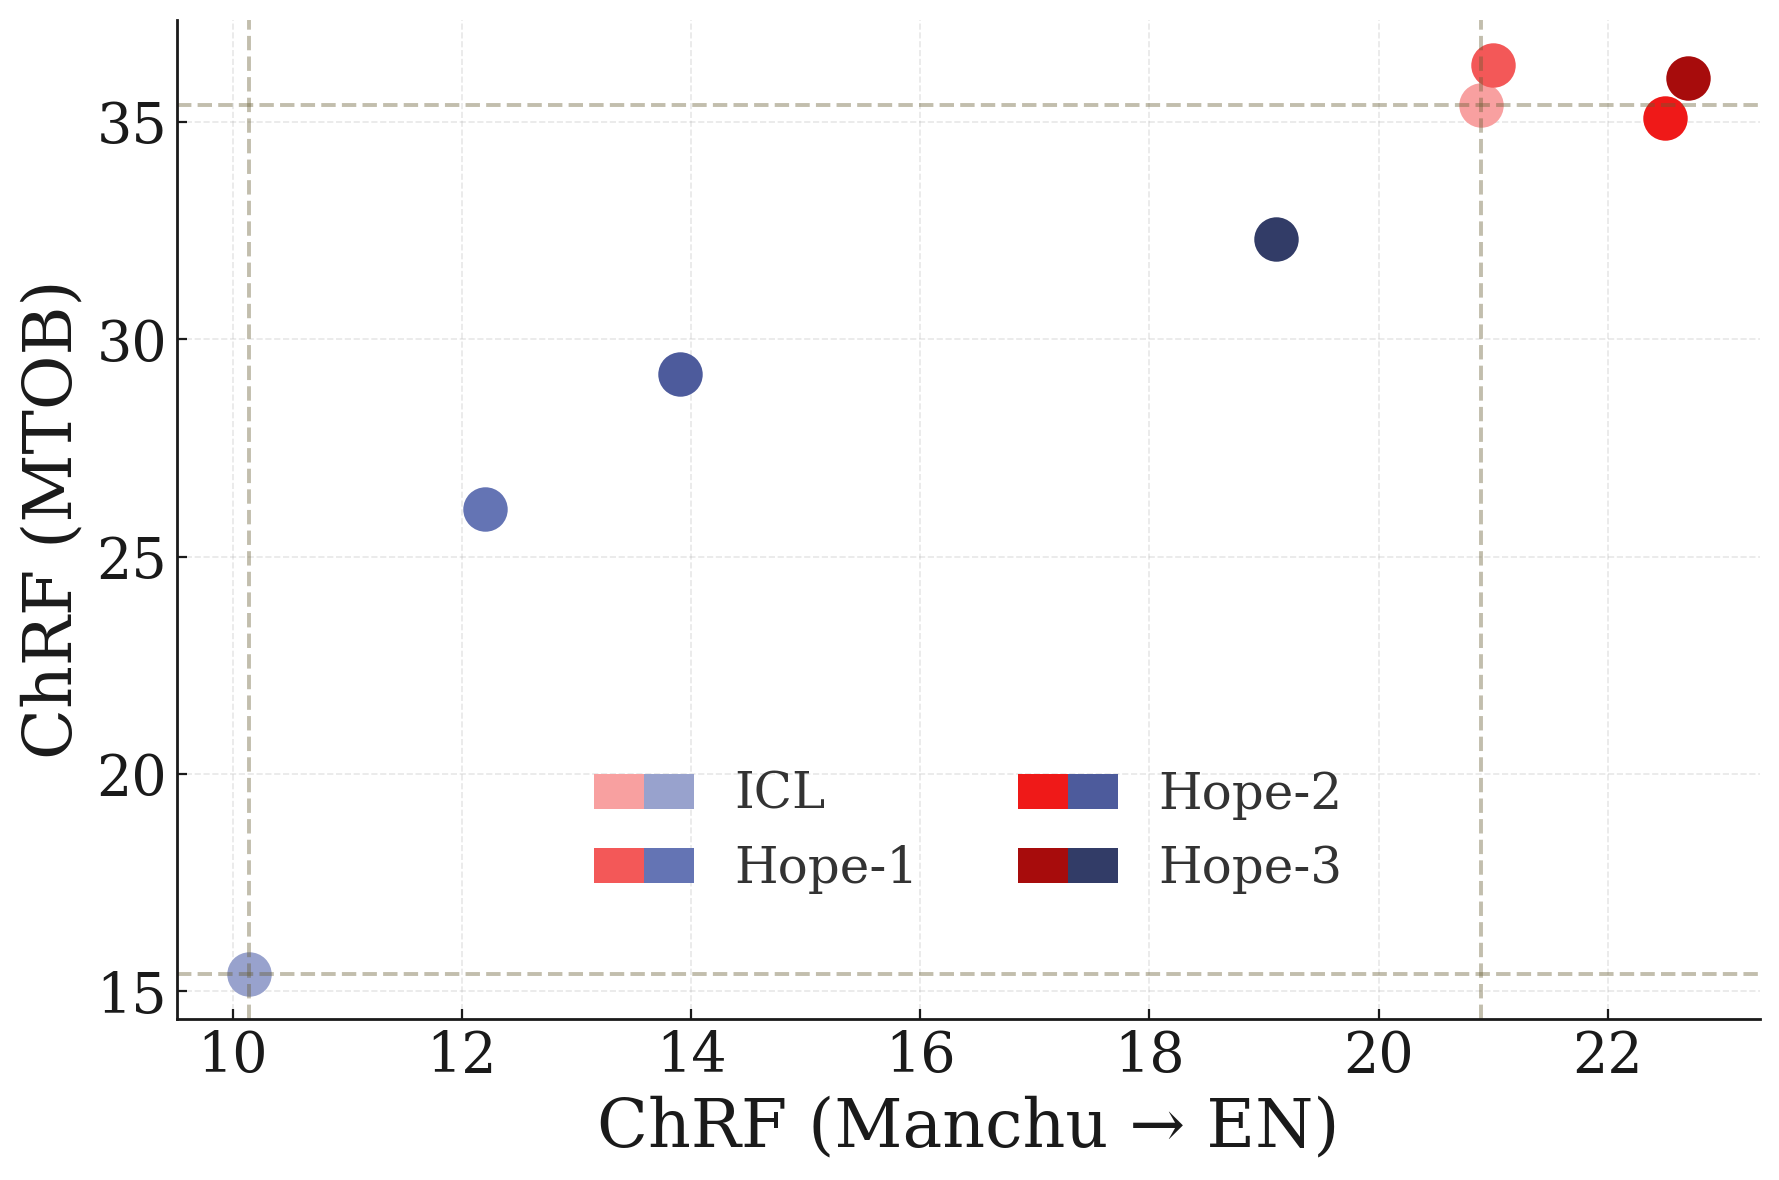
\includegraphics[width=\linewidth]{Images/ICL-Translate.png}
                \captionof{figure}{Continual Translation of a Novel Language (CTNL) task. \textcolor{darkred}{Red} points are the results with only one language.  \textcolor{darkblue}{Blue} points are the results in the continual leanring setup.}
                \label{fig:icl-translate}
            \end{minipage}
            \vspace*{10ex}
            \begin{minipage}{\linewidth}
                \centering
                \vspace{1ex}
                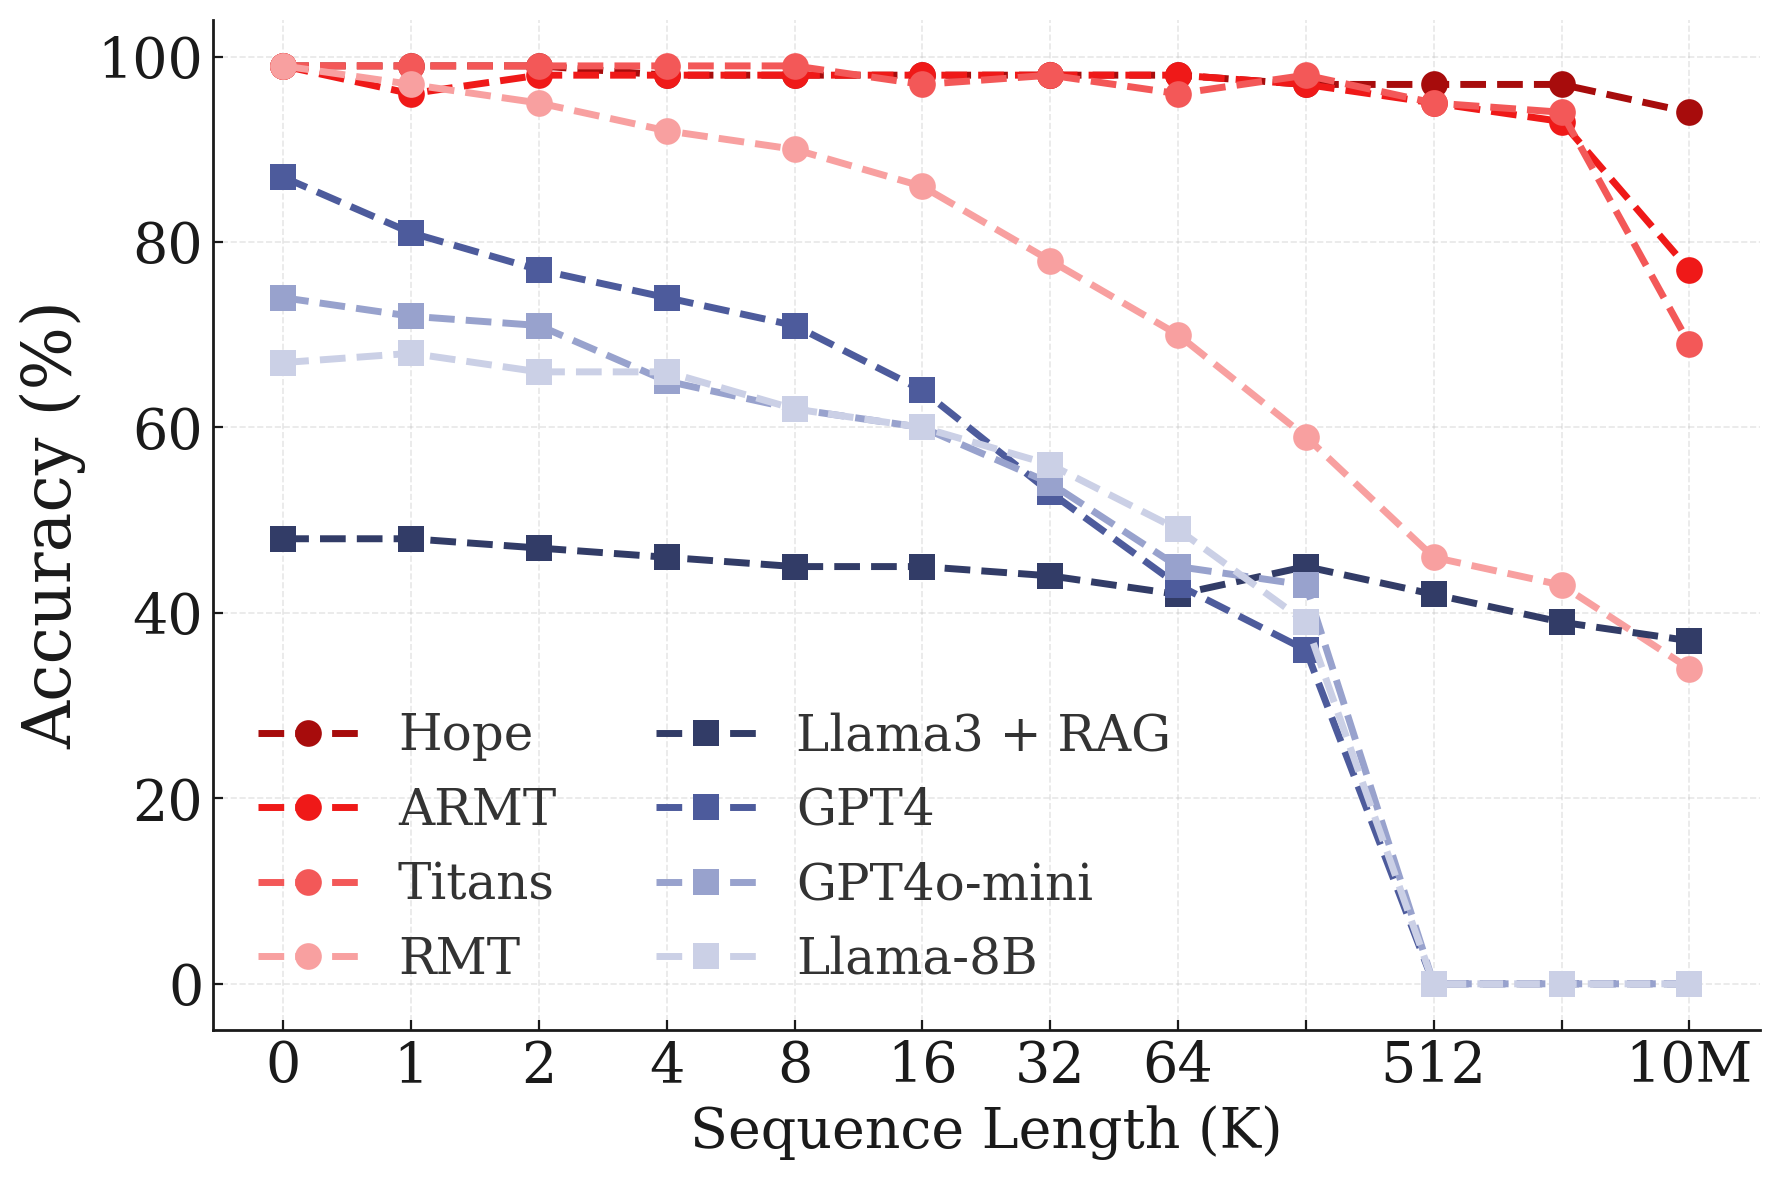
\includegraphics[width=\linewidth]{Images/BABILong.png}
                \captionof{figure}{BABILong Benchmark. \textcolor{darkred}{Red} points are the results of fine-tuned models, and \textcolor{darkblue}{Blue} points are the large models' zero-shot results. }
                \label{fig:babilong}
                \vspace{-7ex}
            \end{minipage}
    \end{minipage}
\end{table*}


The results are reported in \autoref{fig:effect-level}. \model{} with any number of levels and also with any lowest frequency outperforms both ICL baseline as well as the efficient DuoAttention. Furthermore, comparing the \model's variants with themselves, the results suggest that: (1) The more levels of memory can help with in-context learning capability of the model and enhances its long-term memory and so long-context understanding;  and (2) The higher the lowest-frequency the lower the performance. As discussed above, the lowest-frequency memory is the most persistent memory of the model and so increasing it means that the model has a weaker but more adaptive long-term memory. Due to the fact that the frequency of update directly affects the efficiency of the model, one might find ``Lowest Frequency = 2K'' an optimal setup as it offers significantly more efficient forward pass, while achieves close performance with ``Lowest Frequency = 512''. 






\head{Learning a New Language In-Context}
Throughout the paper, we argued that pre-training can be seen as an in-context learning process, where the context is the entire pre-training data. Accordingly, when we use more levels in the neural learning module, or performing in-context learning on different context flows, we expect the model to show better adaptability and continual learning capabilities. To this end, with combining two existing benchmarks of MTOB~\citep{tanzer2024a} and Manchu~\citep{pei2025understanding}, we design a new continual learning task that the LLM learns two new languages in context and is expected to translate phrases to English. 
Then for our Continual Translation of a Novel Language (CTNL) task, we consider two setups: (1) Learning and testing the performance of the model on each language separately (in \textcolor{darkred}{red} color). This is a baseline we use to measure the catastrophic forgetting when comparing with the next setting; and (2) The model, first, learns these two languages in a sequential manner (in \textcolor{darkblue}{blue} color) and then is asked to translate the phrases to English. We use ICL as the baseline, and to study the importance of multi-level design of \model, we use different variants of \model{} with 1, 2, and 3 additional levels of memory, which we refer to as \model-1, \model-2, and \model-3, respectively.

The results are reported in \autoref{fig:icl-translate}. More specifically, each point is the performance of one model in one of the setups such that the $\vx$-axis (resp. $\vy$-axis) indicates the model ChRF in translation of Manchu $\rightarrow$ English (resp. Kalamang $\rightarrow$ English). In the first setup (in-context translation without continual learning), all \model's variants performs better or on-par compared to ICL, supporting the importance of CMS design. In the second setup (i.e., continual translation), however, ICL faces dramatic performance drop and almost rely on its capabilities achieved in its pre-training (i.e., catastrophic forgetting about the knowledge in the context). On the other hand, increasing the memory levels in the \model{} shows clear improvement and \model-3 almost recovers the ICL capability in the first setup, without continual learning. These results further support the importance of CMS design in continual learning and the ability of the model to adapt itself to the new tasks. 








\subsection{\model: Long Context Understanding}\label{sec:exp-niah}
In the previous section, we evaluated the performance of \model-Attention, when the MLP blocks are adapted to perform in-context learning. In this part, we evaluate the performance of \model{} in long context understanding, when it starts learning from scratch. To this end, we use about 50B tokens from a mixture of FineWeb-Edu~\citep{penedo2024fineweb} and long-context documents with a vocabulary size of 32K to train all the models from scratch. All models are optimized using AdamW with tuned learning rate for each model and with the default optimizer configuration in \citet{behrouz2024titans}. We focus on two popular benchmarks of RULER~\citep{hsieh2024ruler} and BABILong~\citep{kuratov2024babilong}:




\head{Needle-in-a-Haystack (NIAH) Tasks}
In the first part, we focus on the needle-in-a-haystack with different setups of: (1) single needle but different types (i.e., pass-key, number, and uuid), (2) multi-key, (3) multi-query, and (4) multi-value, all follows \citet{hsieh2024ruler}. As for the baselines, we use RetNet~\citep{sun2023retentive} and DeltaNet~\citep{schlag2021linear} as the representative of the models \emph{purely} based on Hebbian- and Delta-rule, and experimented with diverse set of modern \emph{linear} recurrent models and so used the linear models with the best performance: i.e., RWKV-7~\citep{rwkv-repo} and Comba~\citep{hu2025improving}. As another group of baselines, we also compare with \emph{deep} memory modules with dot-product and $L_2$ regression objectives: i.e., DLA~\citep{behrouz2025atlas}, and Titans~\citep{behrouz2024titans}.

The results are reported in \autoref{tab:ruler}. Comparing with other attention-free models, \model{} achieves the best performance across all tasks and levels of difficulties. Particularly, comparing to linear memories, deep memory modules show better performance in longer sequences, mainly due to their higher memory capacity to compress more tokens. Comparing \model{} with Titans, the superior performance of \model, specifically in longer context length supports the importance of both self-referential update as well as the CMS design. Finally, we also evaluate the performance of \model-Attention and compare it with Transformers to better understand the contribution of CMS design. The results indicate that \model-Attention achieves a better performance compared to Transformers, supporting the advantage of having CMS in \model-Attention design. 







\head{BABILong} Next, we evaluate the \model's performance on BABILong benchmark~\citep{kuratov2024babilong} and compare it with (1) large models such as GPT4 and GPT4o-mini~\citep{achiam2023gpt}; (2) middle-size Llama-8B model~\citep{dubey2024llama} with its RAG augmented version; and (3) the state-of-the-art small models in this tasks: i.e., RMT~\citep{bulatov2022recurrent}, ARMT~\citep{rodkin2024associative}, and Titans~\citep{behrouz2024titans}. We follow the original setup of the benchmark and fine-tune the small models with the same process as \citet{kuratov2024babilong}. 


The results are reported in \autoref{fig:babilong}. Large models show significant performance drop with increasing the sequence length, where all fail around 128K-256K context length. The RAG augmented model also show a drop with increasing the context, but it is able to relatively maintain its performance after 256K context length. Among fine-tuned models, Titans, ARMT, and \model{} show competitive results until 1M context length, but the performance of both Titans and ARMT drop fast after that point. \model{} maintains its good performance even for 10M context length, mainly due to its CMS design. It is notable that the performance of all small models, including \model, can drop significantly when used without fine-tuning. The reason is, compressing large context (e.g., 10M), in addition to a powerful memory management in the high-frequency level, requires enough capacity to compress 10M tokens or at least tokens that are needed for the final answer. The fine-tuning step helps the models to adjust their lower-frequency levels to adapt fast and so properly manage their memory in the higher-frequency levels.   


























































\begin{table*}[t!]
\centering
\caption{
Performance of models on language modeling and common-sense reasoning tasks.
}\label{tab:lm_results}
\centering
\resizebox{0.85\linewidth}{!}{
\centering
\begin{tabular}{l|c c|c c c c c c c c c}
\toprule
\textbf{Model}  & \textbf{Wiki.}  &  \textbf{LMB.} &  \textbf{LMB.} & \textbf{PIQA} &    \textbf{Hella.} & \textbf{Wino.} & \textbf{ARC-e} &  \textbf{ARC-c} &  \textbf{SIQA}  & \textbf{BoolQ} &  \textbf{Avg.} \\
 & ppl $\downarrow$  &  ppl $\downarrow$  &  acc $\uparrow$  & acc $\uparrow$ &   acc\_n $\uparrow$  & acc $\uparrow$  & acc $\uparrow$ & acc\_n $\uparrow$ &  acc $\uparrow$  & acc $\uparrow$ &   $\uparrow$  \\
\midrule
\midrule
\multicolumn{12}{c}{760M params / 30B tokens} \\
\midrule
 Transformer++ & 24.18 & 24.27 & 37.1 & 67.2 & 43.8 &	53.0 & 65.6	& 33.4 &  39.1  & 61.7  & 50.11 \\
 Samba$^{*}$ & 21.07 & 22.85 & 39.2 & 68.9 & 47.8 &	53.1 & 65.8	& 34.9 &  38.9  & 63.1  & 51.46 \\
 \midrule
 RetNet & 25.77 & 24.19 & 34.5 & 66.8 & 41.2 &	51.9 & 63.6	& 32.5 &  38.8  & 56.2  &  48.19\\
 DeltaNet & 24.52 & 24.38 & 36.8 & 67.3 & 44.5 &	51.8 & 64.2	& 32.7 &  39.6  & 60.1  & 49.63 \\
 RWKV-7 & 23.75 & 23.08 & 37.1 & 67.3 & 47.6 & 52.2 & 64.7 & 34.2 & 39.4 & 61.9 & 50.55\\
 Comba & 22.41 & 22.19 & 37.5 & 66.9 & 48.2 & 52.4 & 65.1 & 34.1 & 40.1 & 62.8 & 50.89 \\
  \midrule
   TTT & 24.17 & 23.51 & 34.7 & 67.3 & 43.9 & 51.0 & 64.5 & 33.8 & {40.2} & 59.6 & 47.32 \\
 Miras (Memora) &  22.28 & 22.31 & 38.2 & 67.8  & 49.3 & 53.3 & 63.6 & 36.1 & 40.9 & 63.0 & 51.53\\
 DLA &  23.12 & 22.09  &  36.1   &  68.0 &  47.9 &  52.7 & 65.8  & 34.6 & 39.1 & 59.6 &  50.48\\
Titans & 20.08 & 21.52 & 38.1 & 69.1  & 48.5 & 52.7 & 66.2 & 35.7 & 40.3 & 62.8 & 51.68\\
\midrule
\rowcolor{mygray} \model & 18.68 & 20.07 & 38.8 & 69.2  & 49.1 & 53.6 & 66.8 & 36.1 & 41.2 & 63.4 & 52.28\\
  \toprule
\multicolumn{12}{c}{1.3B params / 100B tokens} \\
\midrule
 Transformer++ & 17.92 & 17.73 & 42.6 & 71.4 & 52.3 &	54.1 & 69.9	& 36.5 &  41.8  & 58.4  & 53.38\\
 Samba$^*$ & 16.15 & 13.21 & 45.2 & 71.5 & 53.8 &	55.8 & 69.1	& 36.7 &  40.6  &  {63.0}  & 54.46 \\
 \midrule
 RetNet & 18.91 & 17.04 & 41.2 & 71.3 & 49.1 &	55.2 & 67.5	& 34.1 &  {41.4}  & {61.0}  & 52.60 \\
 DeltaNet & 18.62 & 17.10 & 41.6 & 70.1 & 49.4 &	52.7 & 67.6	& 35.2 &  39.7  & 54.8  & 51.39 \\
 RWKV-7 & 18.44 & 15.96 & 46.7 & 72.4 & 54.9 & 57.5 & 71.6 & 38.2 & 40.7 & 60.4 & 55.30\\
 Comba & 18.16 & 14.87 & 46.9 & 73.1 & 54.5 & 57.7 & 72.0 & 39.1 & 40.2 & 60.6 & 55.39 \\
\midrule
TTT & 18.42 & 14.51 &  46.8 & 72.9  & 55.2 &  59.0 & 71.8 & 39.5 &  39.8 & 59.6 & 55.58 \\
 Miras (Memora) &  15.90 & 12.04  &  48.7   &  73.1 &  56.0 &  57.4 & 71.5  & 37.9 & 40.2 & 61.3 &  55.76\\
DLA & 16.31 & 12.29 & 44.5   & 70.6 & 53.9 & 54.2 & 69.6 & 36.0 & 40.8  & 60.2 & 53.72\\
Titans & 15.60 & 11.41 &  49.1 & 73.1  & 56.3 &  59.8 & 72.4 & 40.8 &  42.1 & 61.0 & 56.82\\
\midrule
\rowcolor{mygray} \model & 14.39 & 10.08 &  51.0 & 73.9 & 57.5 & 61.2 & 73.8 & 42.7 & 42.8 & 61.4 & 58.04 \\
\bottomrule
\multicolumn{5}{l}{$^*$ is a hybrid of attention + linear RNN~\citep{ren2024samba}.}
\end{tabular}
}
\end{table*}










\subsection{\model: Language Modeling and Common-Sense Reasoning}\label{sec:exp-lm}
In this section, we aim to study \model{} as a backbone of a language model and evaluate it on common language modeling and common-sense reasoning tasks with the setup of: 
\begin{itemize}
    \item Datasets: We evaluate \model{} and baselines on Wikitext~\citep{merity2017pointer}, LMB~\citep{paperno-etal-2016-lambada}, PIQA~\citep{bisk2020piqa}, HellaSwag~\citep{zellers-etal-2019-hellaswag}, WinoGrande~\citep{sakaguchi2021winogrande},  ARC-easy (ARC-e) and ARC-challenge (ARC-c)~\citep{clark2018think}, SIQA~\citep{sap-etal-2019-social}, and BoolQ~\citep{clark-etal-2019-boolq} benchmarks.
    \item {Baselines}: As for the baselines, similar to \autoref{sec:exp-niah}, we use RetNet~\citep{sun2023retentive} and DeltaNet~\citep{schlag2021linear} as the representatives of the models that are \emph{purely} based on Hebbian- or Delta-rule, and two modern \emph{matrix-valued} recurrent models with the best performance compared to others: i.e., RWKV-7~\citep{rwkv-repo} and Comba~\citep{hu2025improving}. As another group of baselines, we compare with attention-free \emph{deep} memory modules with diverse internal attentional bias of dot-product, $L_2$, and $L_p$ regression: i.e., TTT~\citep{sun2024learning}, Miras~\citep{behrouz2025Miras}, DLA~\citep{behrouz2025atlas} and Titans~\citep{behrouz2024titans}. Finally, we also compare with Transformers~\citep{transformers, dubey2024llama} as well as the hybrid of attention and linear RNN, Samba~\citep{ren2024samba}. 
    \item Training: We train models with about 760M and 1.3B parameters, trained with 30B and 100B tokens, respectively, from a mixture of FineWeb-Edu~\citep{penedo2024fineweb} and long-context documents with a vocabulary size of 32K to train all the models from scratch. All models are optimized using AdamW with tuned learning rate for each model and with the default optimizer configuration in \citet{behrouz2024titans}.
\end{itemize}
The results are reported in \autoref{tab:lm_results}. \model{} outperforms all the baselines on the average performance in both language modeling and common-sense reasoning benchmarks. Interestingly, with scaling the parameters, \model{} show higher performance gain compare to other attention-free models. 








\subsection{\model: In-context Recall Tasks and MAD Synthetic Benchmark}\label{sec:retrieval-tasks}
In-context recall is often referred to as one of the challenging benchmarks for attention-free models. In this section, we follow \citet{arora2024simple} and perform experiments on SWDE~\citep{lockard2019openceres}, NQ~\citep{kwiatkowski2019natural}, DROP~\citep{dua2019drop}, FDA~\citep{arora2023language}, SQUAD~\citep{rajpurkar2016squad}, and TQA~\citep{kembhavi2017you} to evaluate the effectiveness of \model's design. We use the same set of baselines and experimental setup as the above previous section. The results are reported in \autoref{tab:recal}. Transformers achieve the best performance, while \model{} show competitive results, outperforming all the attention-free baselines and closing the gap with Transformers. 


\begin{minipage}[t]{0.48\textwidth}
    \centering
    \captionof{table}{The performance of \model{} and baselines in short in-context recall tasks. \model{} outperforms all attention-free models and close the gap with Transformers.}
    \label{tab:recal}
    \resizebox{\linewidth}{!}{
    \begin{tabular}{l c c c c c c }
    \toprule
         &  \multirow{1}{*}{SWDE} & \multirow{1}{*}{NQ} & \multirow{1}{*}{DROP} & FDA & SQUAD & \multirow{1}{*}{TQA} \\
         \midrule
         \midrule
        Transformers & 71.4 & 22.0 & 23.9 & 67.3 & 39.4 & 59.1 \\
        RWKV-7 & 52.3 & 17.8 & 21.7 & 32.8 & 28.5 & 56.2 \\
        Comba & 53.9 & 19.1 & 21.9 & 35.5 & 30.2 & 56.4 \\
        Titans & 60.8 & 20.3 & 22.0 & 37.6 &  31.8 & 57.5 \\
                 \midrule
        \rowcolor{mygray} \model{} & 65.9 &  21.2 & 22.8 & 41.9 & 33.0 & 57.7 \\
    \toprule
    \end{tabular}
    }
\end{minipage}~\hspace{1ex}~
\begin{minipage}[t]{0.51\textwidth}
    \centering
    \captionof{table}{Performance of \model{} and baselines on the synthetic benchmark of MAD~\citep{poli2024mechanistic}. \model{} outperforms all the baselines, including Transformers.}
    \label{tab:MAD}
    \resizebox{\linewidth}{!}{
    \begin{tabular}{l c c c c c}
    \toprule
         &  \multirow{2}{*}{Compress.} & \multirow{2}{*}{ICR} & \multirow{2}{*}{Fuzzy ICR} & Selective & \multirow{2}{*}{Memory} \\
         &  & & & Copying \\
         \midrule
         \midrule
        Transformers & 49.4 & 100 & 47.9 & 96.2 & 83.7\\
         RWKV-7 & 45.1 & 100 & 32.8 & 95.6 & 82.2\\
         Comba & 46.3 & 100 & 32.8 & 96.4 & 82.9\\
         Titans & 49.8 & 100 & 50.0 & 99.4 & 83.4 \\
         \midrule
        \rowcolor{mygray} \model & 51.2 & 100 & 52.1 & 99.7 & 85.2\\
    \toprule
    \end{tabular}
    }
\end{minipage}




We also study the performance of \model{} on MAD benchmark~\citep{poli2024mechanistic}, which is a synthetic benchmark, evaluating the performance of models in recall, memorization, compression, and copying tasks. The results are reported in \autoref{tab:MAD}. \model{} achieves the best results compared to baselines. 





\begin{table*}[t]
    \centering
    \small
    \caption{Accuracies of various models on the formal language recognition tasks.}
    \label{tab:formal-language}
    \resizebox{0.95\linewidth}{!}{
        \begin{tabular}{l c rrrrrrrrrrrrr}
        \toprule
         & & \multicolumn{6}{c}{Non-Star-Free Regular} & \multicolumn{6}{c}{\textcolor{black!40!white}{Counter}} \\  \cmidrule(r{.45em} l{.50em}){3-8}  \cmidrule(r{.45em} l{.50em}){9-14}
         & Parallel & \multicolumn{2}{c}{Parity} & \multicolumn{2}{c}{$(aa)^*$}  & \multicolumn{2}{c}{$(abab)^*$} & \multicolumn{2}{c}{\textcolor{black!40!white}{$a^nb^n$}} & \multicolumn{2}{c}{\textcolor{black!40!white}{$a^nb^nc^n$}} & \multicolumn{2}{c}{\textcolor{black!40!white}{Shuffle-2}}\\  \cmidrule(r{.45em} l{.50em}){3-8}  \cmidrule(r{.45em} l{.50em}){9-14}
        Model & Training & Bin0 & Bin1 & Bin0 & Bin1 & Bin0 & Bin1 & \textcolor{black!40!white}{Bin0} & \textcolor{black!40!white}{Bin1} & \textcolor{black!40!white}{Bin0} & \textcolor{black!40!white}{Bin1} & \textcolor{black!40!white}{Bin0} & \textcolor{black!40!white}{Bin1} 
         \\
        \midrule
        LSTM & \xmark & \textbf{100.0} & \textbf{100.0} & \textbf{100.0} & \textbf{100.0} & \textbf{100.0} & \textbf{100.0} & \textcolor{black!40!white}{\textbf{100.0}} & \textcolor{black!40!white}{\textbf{100.0}} & \textcolor{black!40!white}{\textbf{100.0}} & \textcolor{black!40!white}{\textbf{100.0}} & \textcolor{black!40!white}{\textbf{100.0}} & \textcolor{black!40!white}{\textbf{100.0}} \\
        Transformer & \checkmark & 46.4 & 0.0 & 0.0 & 0.0 & 0.0 & 0.0 & \textcolor{black!40!white}{\textbf{100.0}} & \textcolor{black!40!white}{\textbf{100.0}} & \textcolor{black!40!white}{\textbf{100.0}} & \textcolor{black!40!white}{\textbf{100.0}} & \textcolor{black!40!white}{\textbf{100.0}} & \textcolor{black!40!white}{\textbf{100.0}} \\ \midrule
        Linear & \checkmark & 78.1 & 0.0 & 0.0 & 0.0 & 0.0 & 0.0 & \textcolor{black!40!white}{\textbf{100.0}} & \textcolor{black!40!white}{\textbf{100.0}} & \textcolor{black!40!white}{\textbf{100.0}} & \textcolor{black!40!white}{\textbf{100.0}} & \textcolor{black!40!white}{\textbf{100.0}} & \textcolor{black!40!white}{\textbf{100.0}}  \\
        DeltaNet & \checkmark & 98.2 &  10.1 & 0.0 & 0.0 & 0.0 & 0.0 & \textcolor{black!40!white}{\textbf{100.0}} & \textcolor{black!40!white}{\textbf{100.0}} & \textcolor{black!40!white}{\textbf{100.0}} & \textcolor{black!40!white}{\textbf{100.0}} & \textcolor{black!40!white}{\textbf{100.0}} & \textcolor{black!40!white}{\textbf{100.0}} \\
        SRWM & \xmark & \textbf{100.0} & \textbf{100.0} & \textbf{100.0} & \textbf{100.0} & \textbf{100.0} & \textbf{100.0} & \textcolor{black!40!white}{\textbf{100.0}} & \textcolor{black!40!white}{\textbf{100.0}} & \textcolor{black!40!white}{\textbf{100.0}} & \textcolor{black!40!white}{\textbf{100.0}} & \textcolor{black!40!white}{\textbf{100.0}} & \textcolor{black!40!white}{\textbf{100.0}}  \\
        \midrule
          \rowcolor{mygray} \model & \checkmark & \textbf{100.0} & \textbf{100.0} & \textbf{100.0} & \textbf{100.0} & \textbf{100.0} & \textbf{100.0} & \textcolor{black!40!white}{\textbf{100.0}} & \textcolor{black!40!white}{\textbf{100.0}} & \textcolor{black!40!white}{\textbf{100.0}} & \textcolor{black!40!white}{\textbf{100.0}} & \textcolor{black!40!white}{\textbf{100.0}} & \textcolor{black!40!white}{\textbf{100.0}} \\
        \bottomrule
        \end{tabular}
}
\end{table*}

\subsection{Language Recognition Tasks}\label{sec:exp-language}
One of the critical limitations of Transformers is on non-parallelizable tasks, where the recurrence plays a significant rule in achieving proper performance. An example of such tasks is state tracking problem, where the model needs to track its state given a sequence of instructions (movement, etc.), and several studies have shown that Transformers both in theory and practice significantly underperforms models with non-linear recurrence~\citep{merrill2024the, grazzi2025unlocking}. In this section, we focus on formal language recognition tasks and follow the construction of the benchmark by \citet{irie2023practical}. The results are reported in \autoref{tab:formal-language}. \model{} achieves the perfect score on all the tasks, similar to other non-linear recurrent models; e.g., LSTM~\cite{LSTM} and SRWM~\citep{irie2022modern}. The main advantage of \model, however, is the fact that when it is needed, it has parallelizable training and so can scale to larger scales for language modeling tasks.  










\begin{table*}
\begin{minipage}{0.6\linewidth}
    \centering
    \captionof{table}{Ablation Study on \model. All components of \model{} are positively contributing to its performance. }
    \label{tab:ablation}
    \resizebox{0.78\linewidth}{!}{
    \begin{tabular}{l c c}
    \toprule
    \multirow{2}{*}{Model}     & Language Modeling & Reasoning \\
    & ppl $\downarrow$ & acc $\uparrow$ \\
    \midrule
    \midrule
    \rowcolor{mygray} \model{}         &   12.24  &  58.1  \\ 
    \midrule
    w/o DGD                &    13.41     &      56.5     \\
    w/o Momentum           &   13.58  &  56.9  \\
    w/o weight decay            &  13.71   &   57.2  \\
    w/o CMS                     &    13.04      &     57.3     \\
    w/o inner-projection $\vk$  &   13.77  &   56.9  \\
    w/o inner-projection $\vv$  &   13.90  &  55.1   \\
    w/o inner-projection $\vq$  &   12.19  &  57.4   \\
    \toprule
    \end{tabular}
    }
\end{minipage}
~\hfill~
\begin{minipage}{0.37\linewidth}
        \centering
        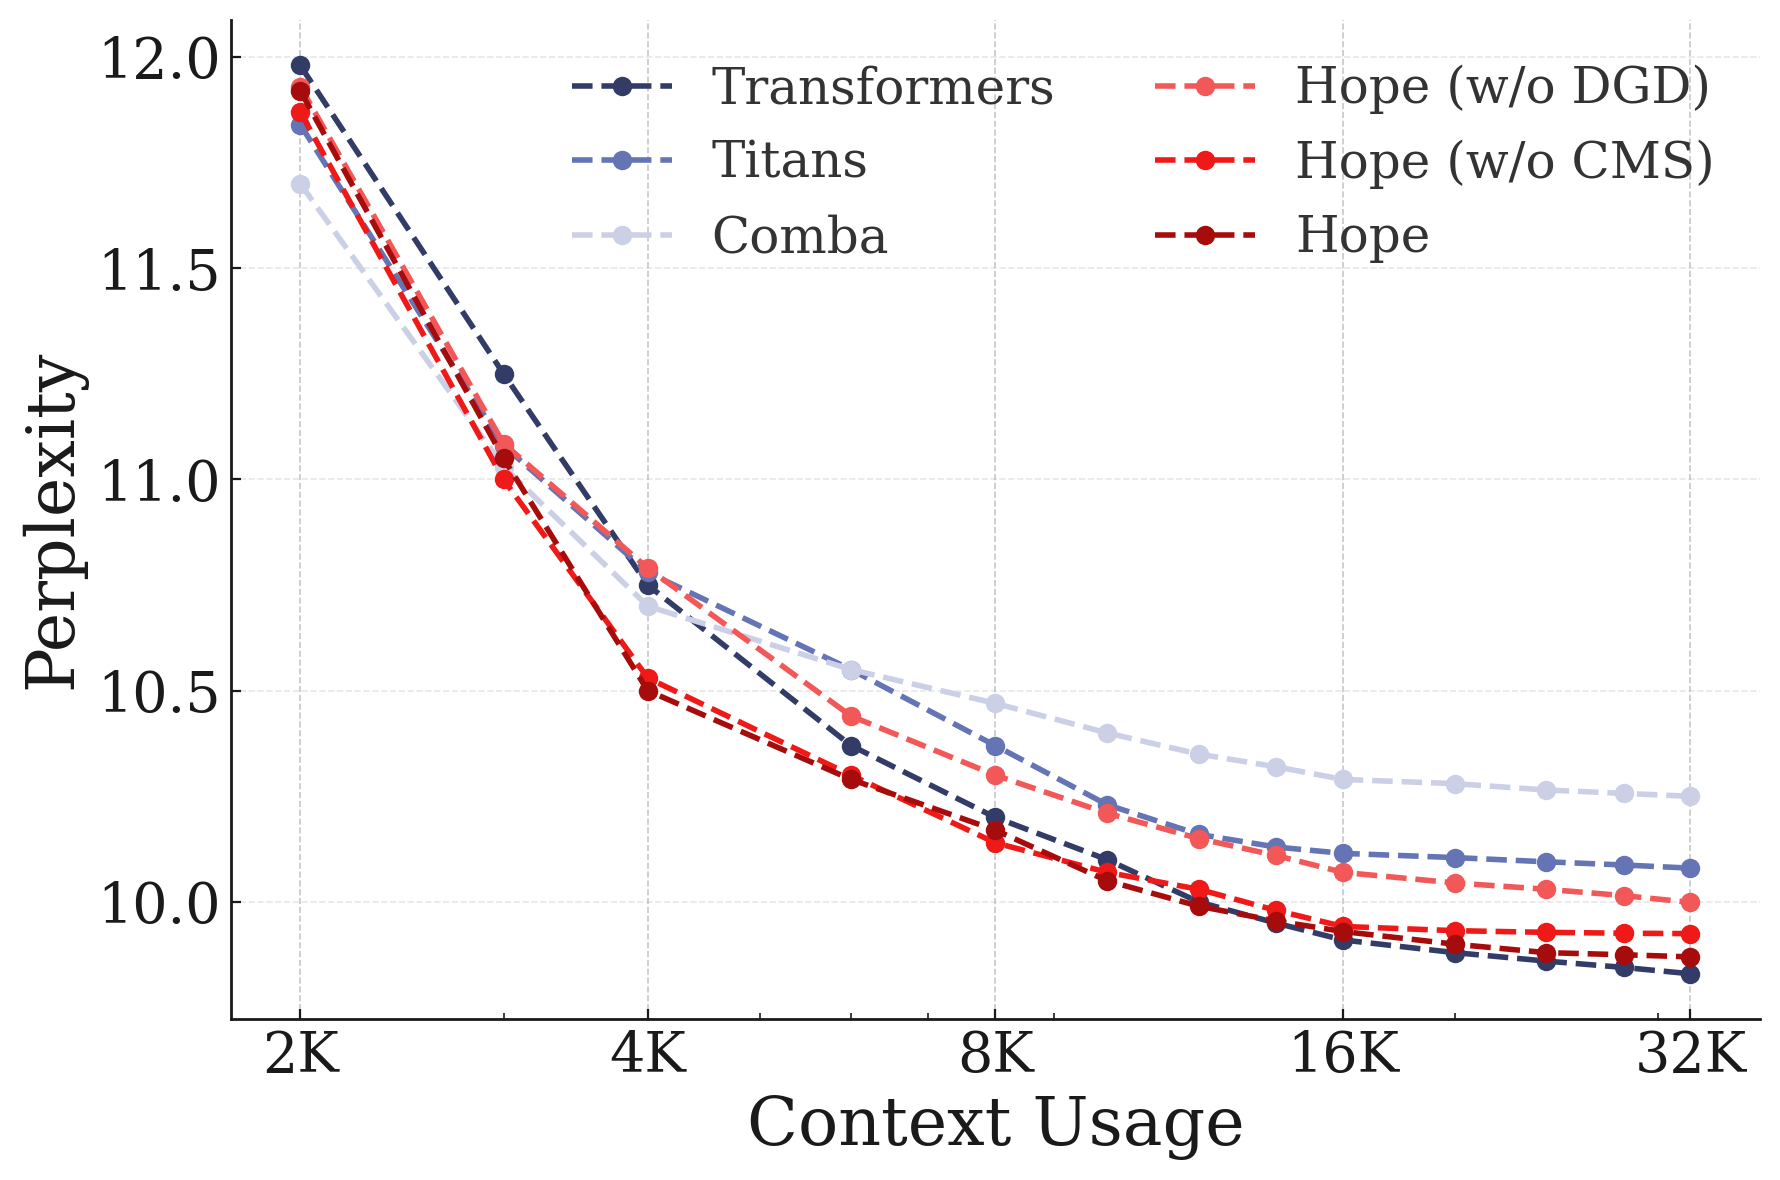
\includegraphics[width=0.87\linewidth]{Images/ablation-context-length.png}
        \captionof{figure}{The effect of context usage on the perplexity of the model. We expect the perplexity of a model with powerful memory management to decrease with more context.}
        \label{fig:placeholder}
\end{minipage}
\end{table*}


\subsection{\model: Ablation Studies and Scaling}
In this section, we first study the importance of design choices we have made for the \model{} architecture by performing ablation studies, where we remove or change one of the \model's components at a time. Note that, in the previous experiments, we have evaluated the significance of some components: E.g., \autoref{fig:icl-translate} and \autoref{fig:effect-level} have already been shown the effect of number of levels as well as the frequency of update on the performance of \model{} in continual learning. In this section, to compare different variants, we use the average perplexity of models in language modeling as well as the average accuracy in common-sense reasoning tasks. The results are reported in \autoref{tab:ablation}. (1) The first row, replaces Delta Gradient Descent with a simple gradient descent in the design of self-modifying Titans; (2) The second row removes the momentum term in the self-modifying Titans; (3) removes the weight decay; (4) removes the CMS from \model's architecture; (5, 6, 7) transfer the projections for $\vk, \vv, \vq$ from higher-frequency level to the lowest-frequency level. All the components of \model{} contribute to its superior performance in these tasks and removing or changing each of them can damage the model's perplexity in language modeling and/or accuracy in common-sense reasoning tasks.  













\begin{table*}
\begin{minipage}{0.612\linewidth}
    \centering
        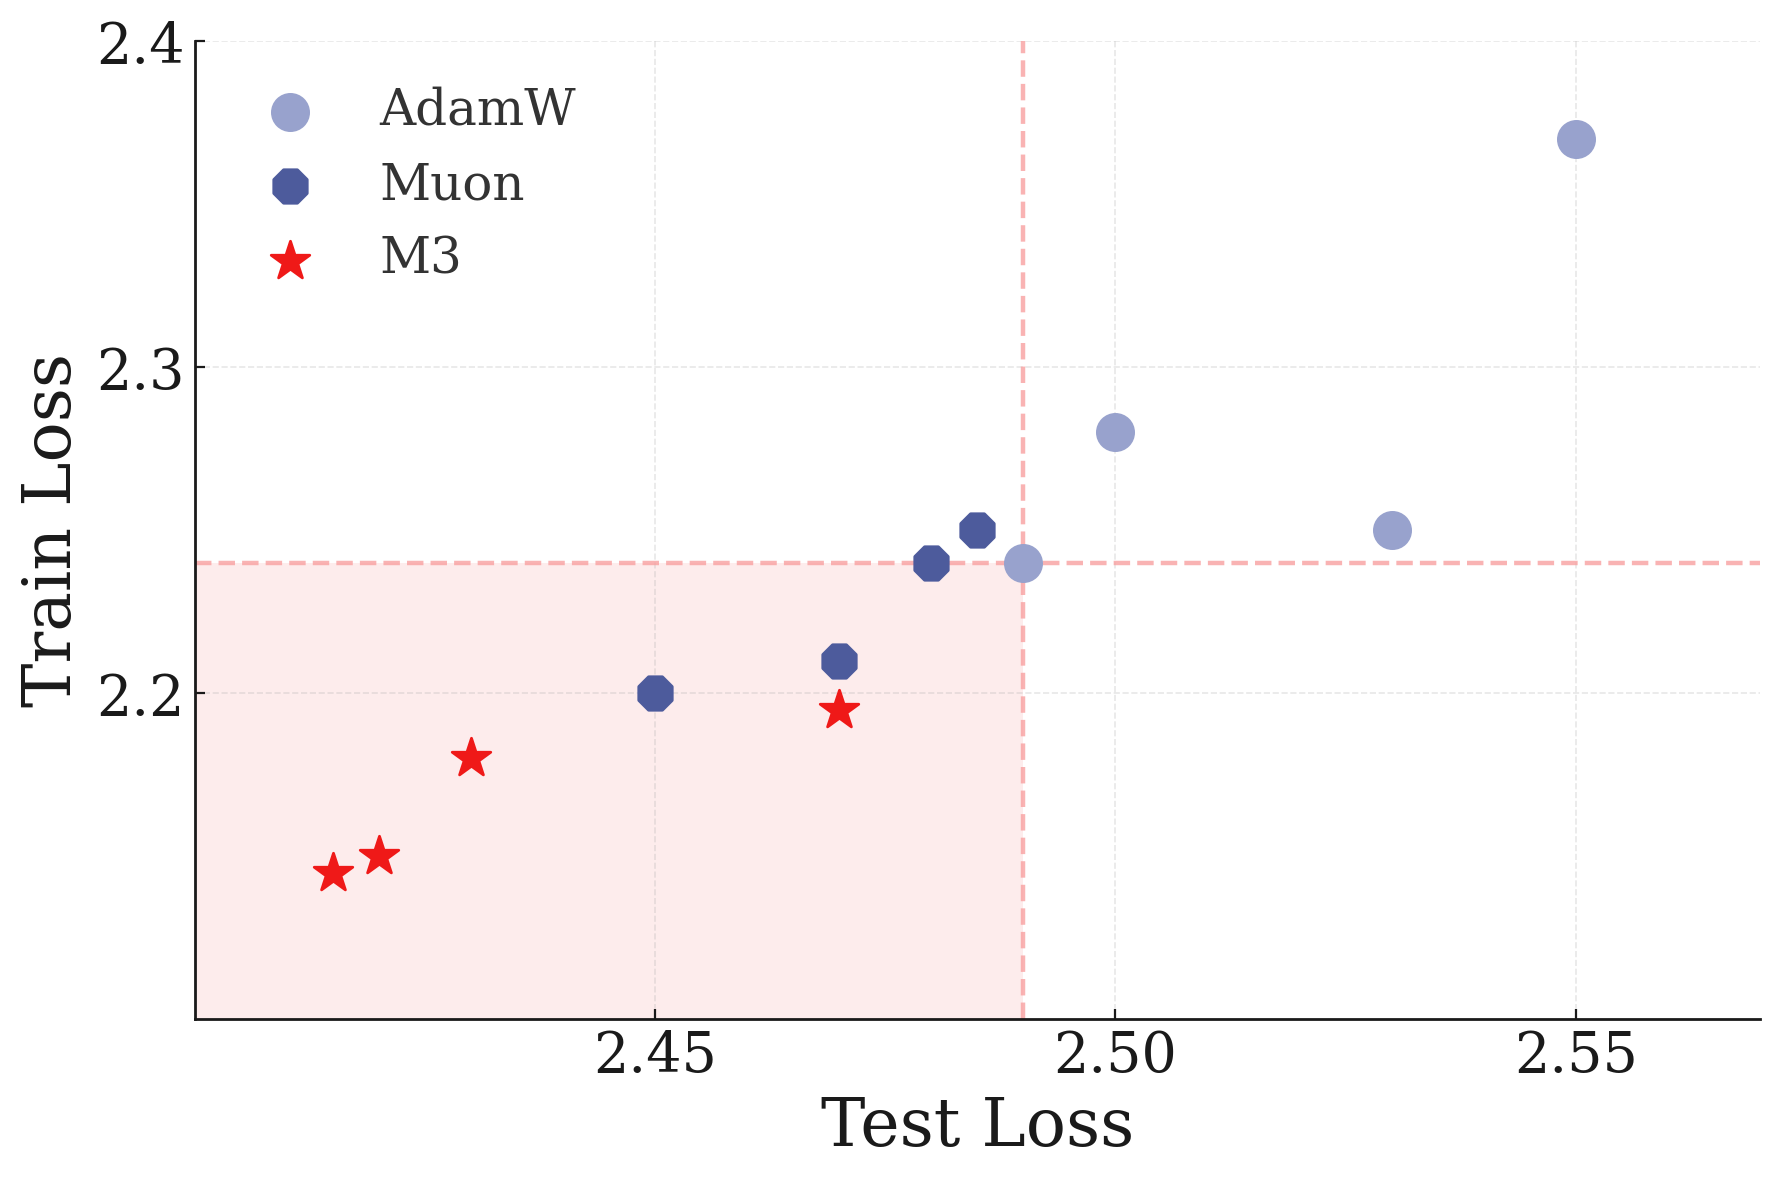
\includegraphics[width=0.5\linewidth]{Images/24M-ImageNet21K.png}~\hfill~
        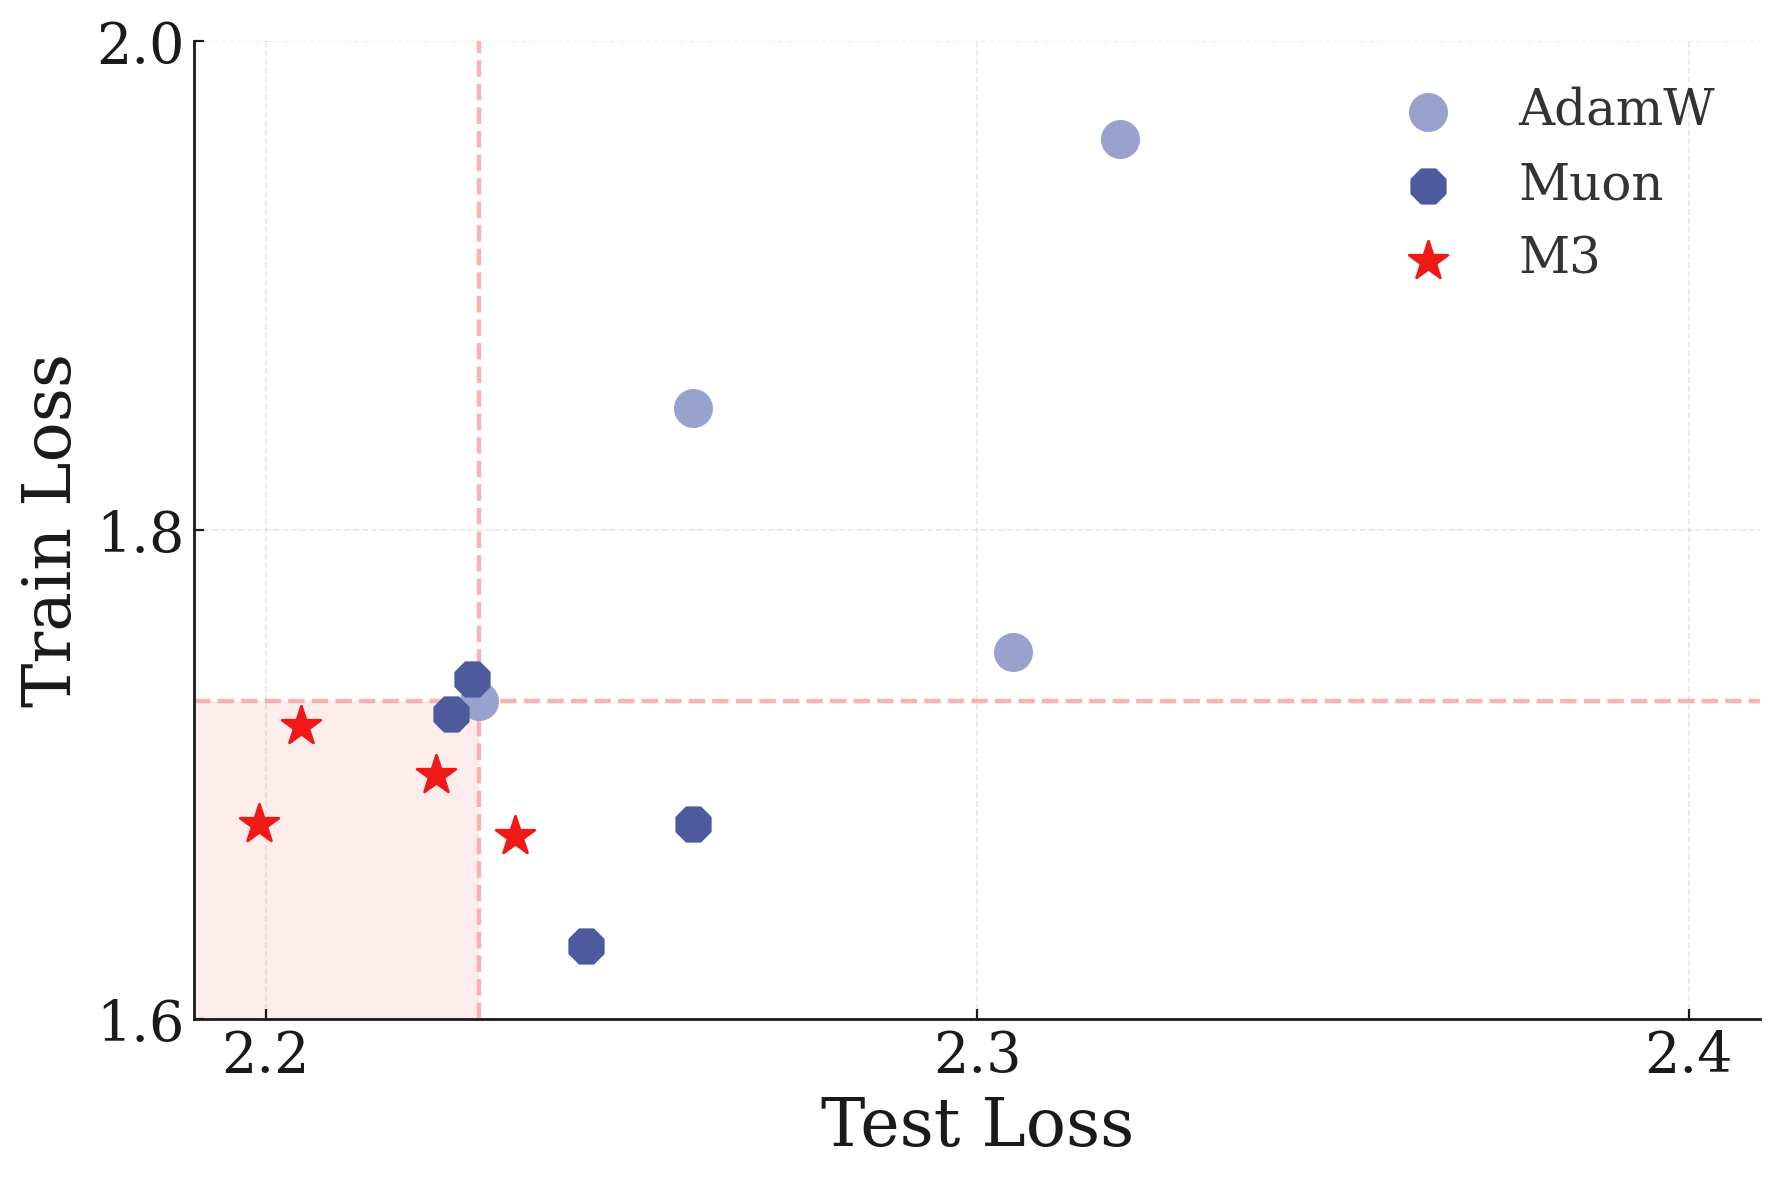
\includegraphics[width=0.5\linewidth]{Images/86M-ImageNet21K.png}
        \captionof{figure}{ViT test and train loss on ImageNet-21K~\citep{ridnik2021imagenetk}, trained with AdamW, Muon, and our M3 optimizers. }
        \label{fig:optimizer-imagenet}
\end{minipage}~\hfill~
\begin{minipage}{0.33\linewidth}
        \centering
        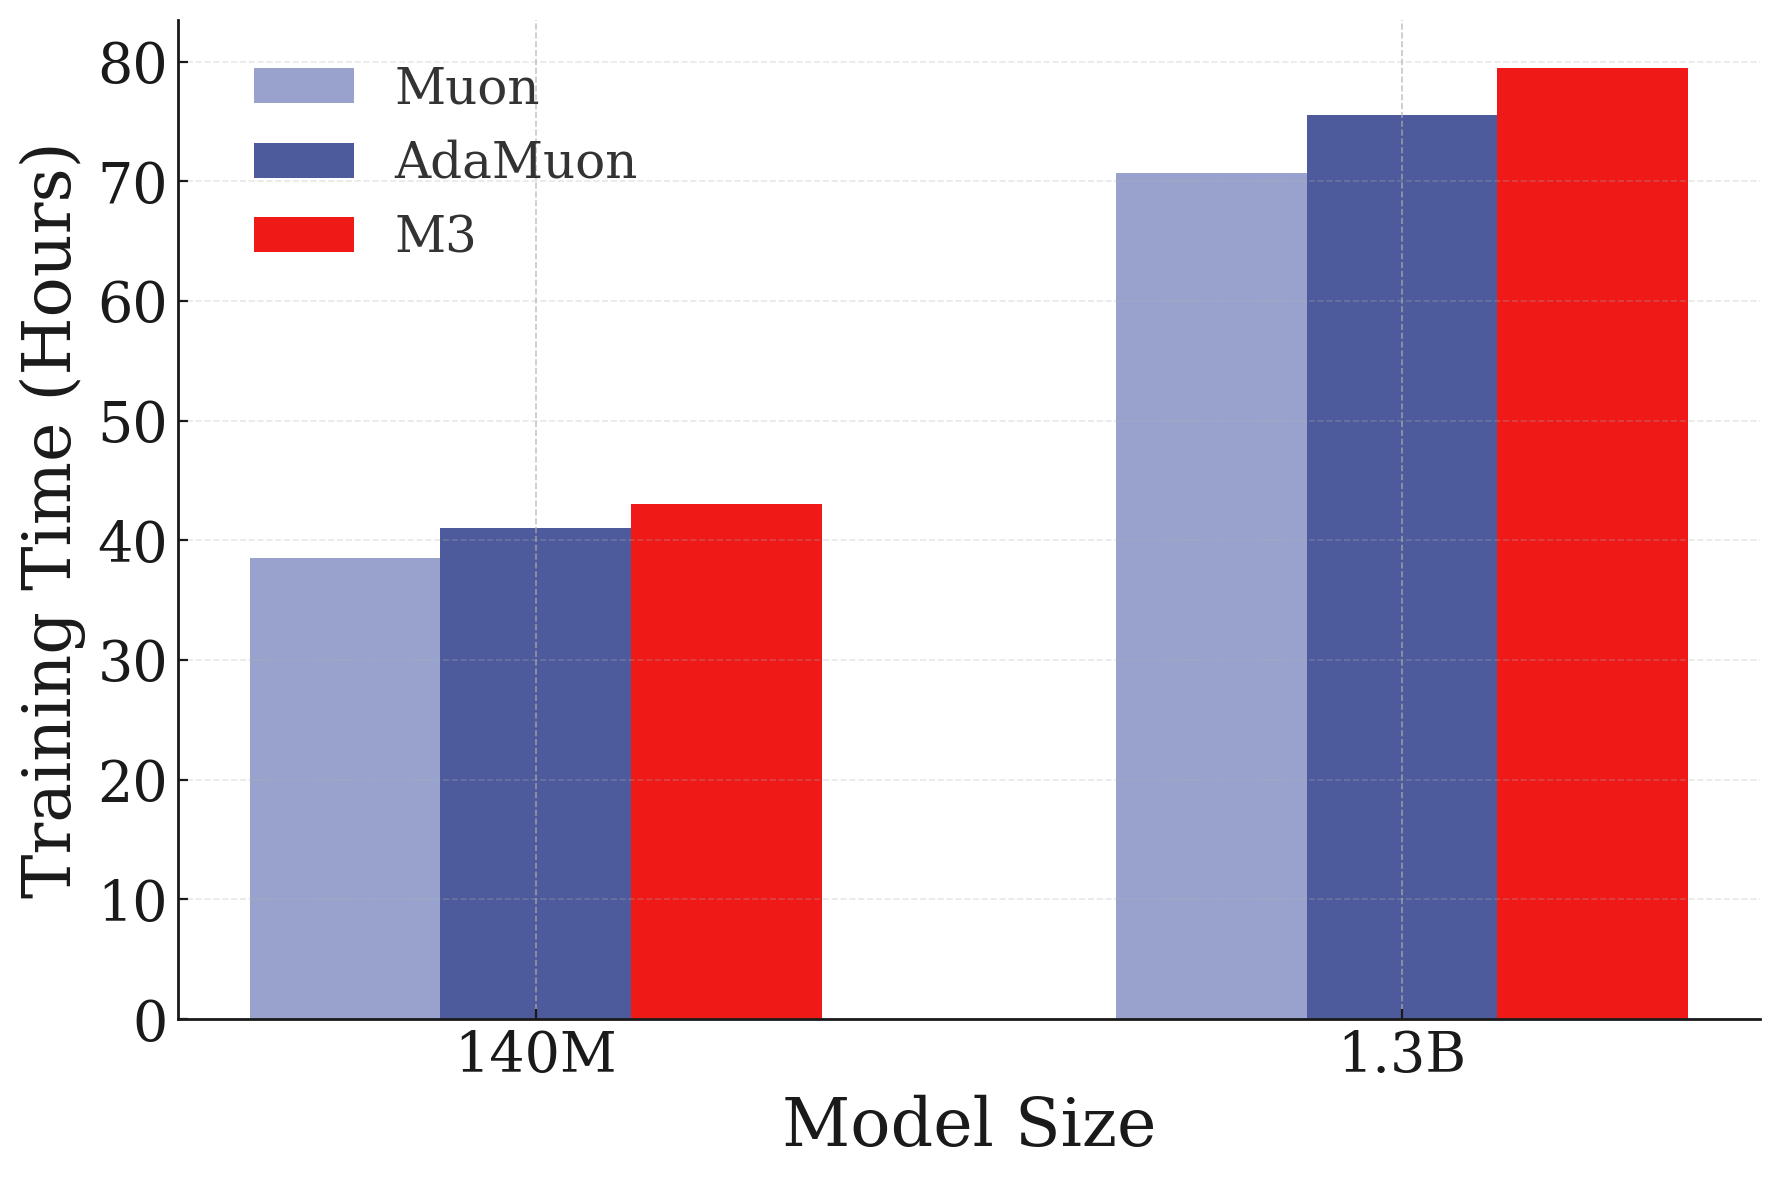
\includegraphics[width=0.92\linewidth]{Images/optimizer-time.png}
        \captionof{figure}{Training time of models with 140M and 1.3B parameters with Muon, AdaMuon, and M3 optimizers. }
        \label{fig:optimizer-efficiency}
\end{minipage}
\end{table*}

\subsection{Expressive Optimizers}\label{sec:exp-deep-optimizer}
In this section, we evaluate the performance of our M3 optimizer from both aspects of effectiveness in finding the solution and also efficiency of training in large scales:

\head{ImageNet} In this experiment, we focus on ViT~\citep{dosovitskiy2021an} architecture for vision tasks and pre-train it on ImageNet-21K, which consists of 11M images corresponding to 10,450 classes. We use a patch size of 16, MLP dimension of 1536 and 3072 for the two scales of 24M and 86M models, respectively. We control all other components and finetuned hyperparameters for each optimizer separately to make sure a fair comparison. We vary the optimizer for training the ViT to understand which of the optimizers find more effective solutions in the same number of training steps. The training and test loss of trained models with different optimizers are reported in Figure~\ref{fig:optimizer-imagenet}. Our M3 shows the best training/test loss compared to both AdamW and Muon. 




\head{Efficiency in Large Models} Due to the small size of the model that is needed for ImageNet, we also perform an efficiency comparison when training a language model. To this end, we use two scales of 140M and 1.3B and train the same Transformer model using different optimizers of Muon~\citep{jordanmuon}, AdaMuon~\citep{si2025adamuon}, and our M3. The results are reported in Figure~\ref{fig:optimizer-efficiency}. Our M3 optimizer, due to the use of multiple momentums (memories) is reletively slower compare to the Muon optimizer, and show on par efficiency with AdaMuon.  





